\documentclass[aspectratio=169]{beamer}

% Default packages
\usepackage[T1]{fontenc}
\usepackage[english]{babel}
\usepackage{csquotes}
\usepackage{pgfplots}
\pgfplotsset{compat=newest}
\usepackage{booktabs}
\usepackage{siunitx}
\usepackage{amsmath}
\usepackage[backend=bibtex,style=authoryear]{biblatex}
\bibliography{bibliography.bib}

% Removes icon in bibliography
\setbeamertemplate{bibliography item}{}

% Font selection
% Latin Modern
\usepackage{lmodern}
% Verdana font type
%\usepackage{verdana}
% Helvetica
%\usepackage{helvet}
% Times (text and math)
%\usepackage{newtx, newtxmath}
% Nice font combination
%\usepackage{mathptmx} % math
%\usepackage{sourcesanspro} % sans-serif
\usepackage{charter} % serif

%Avoid shaded in RMarkdown

% Use DTU theme, see below for options
\usetheme[department=compute]{DTU}

\title[Automated and Early Detection of Disease Outbreaks]{Automated and
Early Detection of Disease Outbreaks}
\author{Kasper Schou Telkamp}
\institute{Section for Dynamical Systems}
\date{2023-02-09}
	
\newcommand{\tabitem}{{\color{dtured}$\bullet$} }

\DeclareMathOperator{\E}{E}
\DeclareMathOperator{\V}{V}
\DeclareMathOperator{\G}{G}
\DeclareMathOperator{\N}{N}
\DeclareMathOperator{\NB}{NB}
\DeclareMathOperator{\Pois}{Pois}
\DeclareMathOperator{\Geom}{Geom}


\begin{document}


\frame{
	\maketitle
}

\frame{
	\frametitle{Outline}
	\tableofcontents
}

\hypertarget{shiga--and-verotoxin-producing-e.-coli.}{%
\section{Shiga- and verotoxin producing E.
coli.}\label{shiga--and-verotoxin-producing-e.-coli.}}

\hypertarget{data-exploration}{%
\subsection{Data exploration}\label{data-exploration}}

\begin{frame}{Data exploration}
\tiny

\begin{table}
\centering\begingroup\fontsize{12}{14}\selectfont

\begin{tabular}{llll}
\toprule
Date & ageGroup & $y_{it}$ & $x_{it}$\\
\midrule
2008-01-01 & <1 year & 2 & 64137\\
2008-01-01 & 1-4 years & 2 & 259910\\
2008-01-01 & 5-14 years & 2 & 680529\\
2008-01-01 & 15-24 years & 1 & 635838\\
... & ... & ... & ...\\
2022-12-01 & 5-14 years & 5 & 634139\\
2022-12-01 & 15-24 years & 1 & 721286\\
2022-12-01 & 25-64 years & 10 & 3031374\\
2022-12-01 & 65+ years & 12 & 1204892\\
\bottomrule
\end{tabular}
\endgroup{}
\end{table}

\normalsize
\end{frame}

\begin{frame}{Data exploration}
\protect\hypertarget{data-exploration-1}{}
\tiny

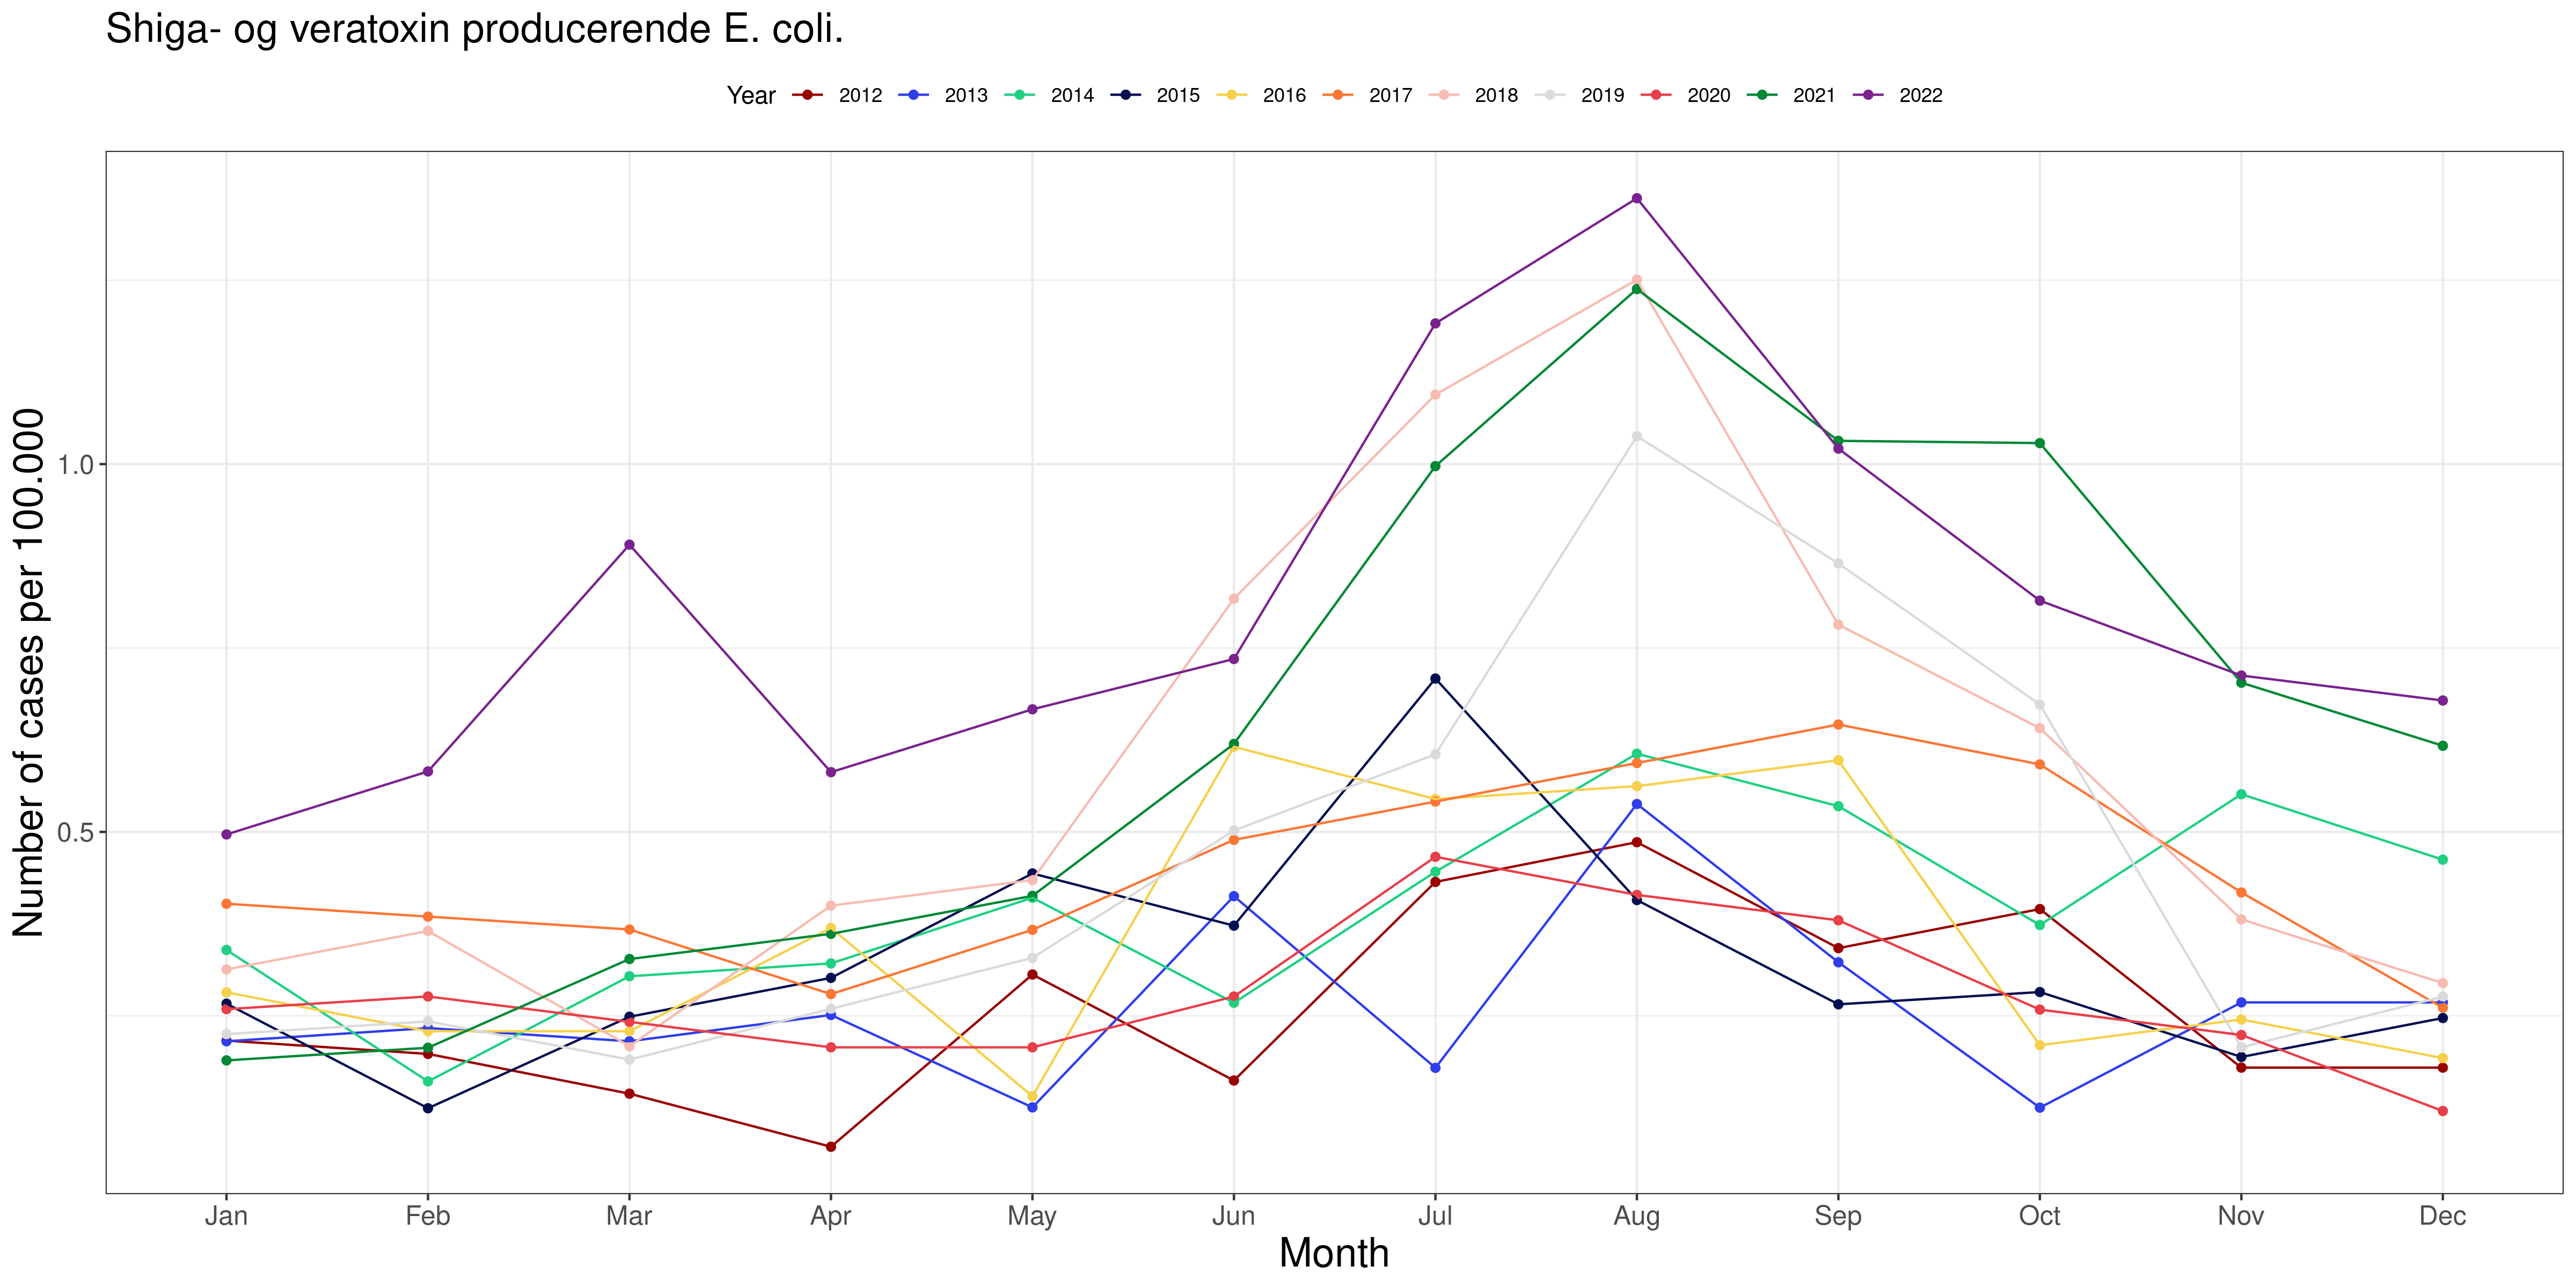
\includegraphics[width=1\linewidth]{../figures/EpixSTEC}

\normalsize
\end{frame}

\begin{frame}{Data exploration}
\protect\hypertarget{data-exploration-2}{}
\tiny

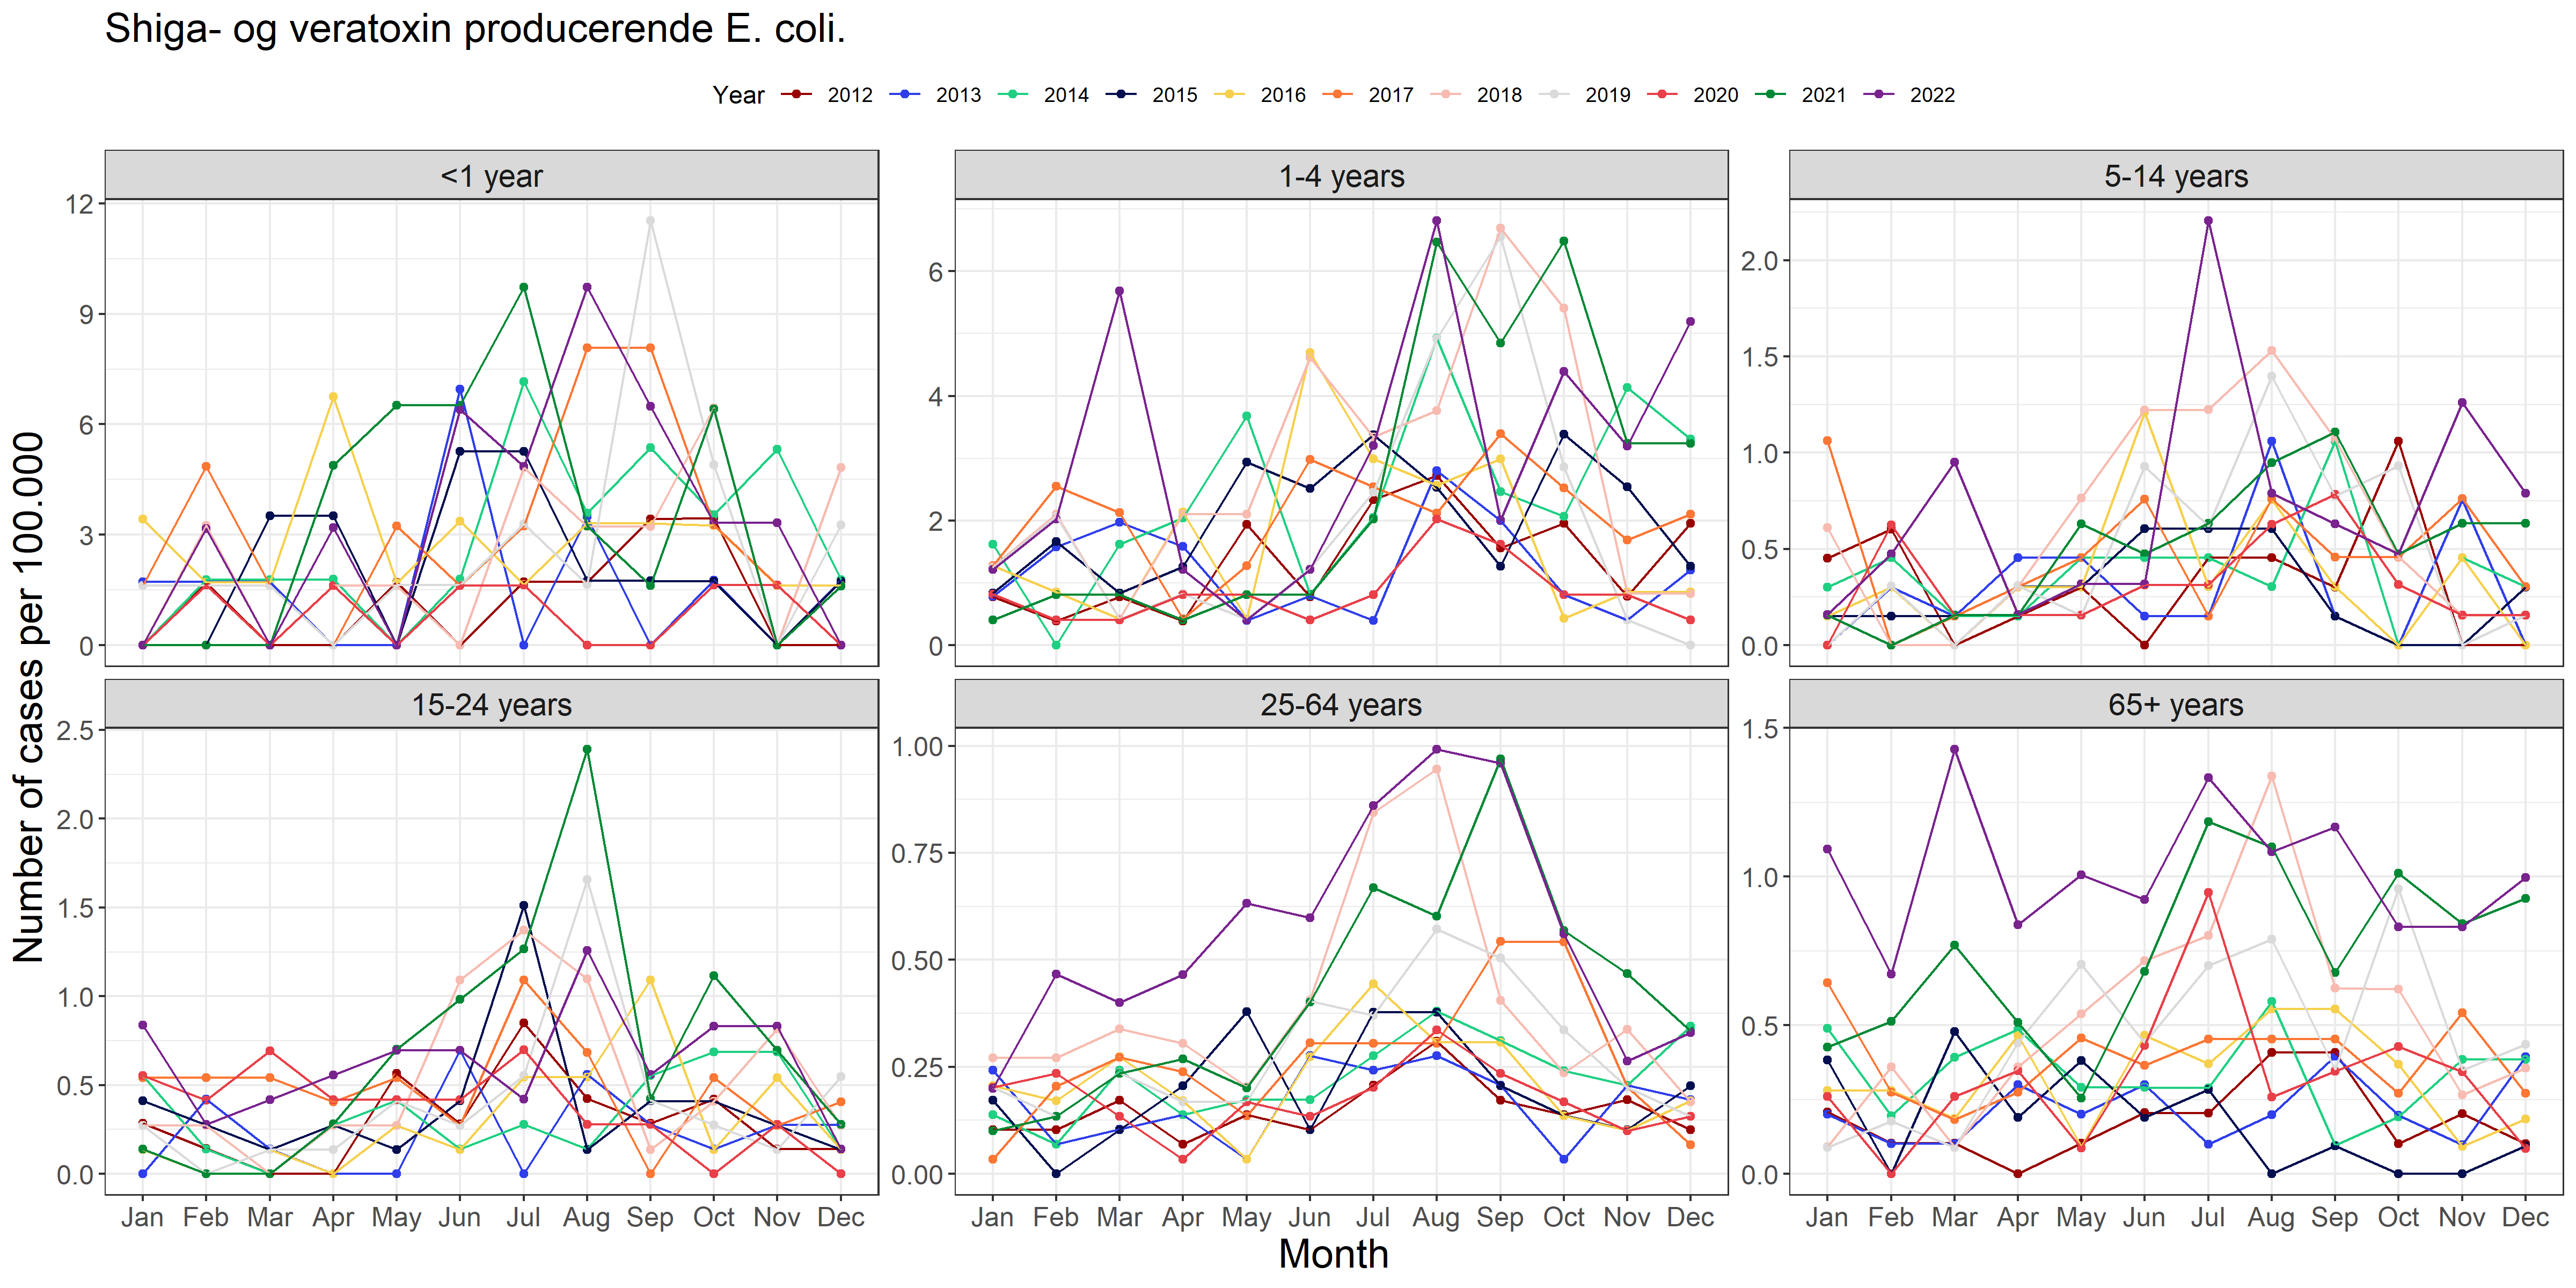
\includegraphics[width=1\linewidth]{../figures/STECxEpixAgeGroup}

\normalsize
\end{frame}

\begin{frame}{Data exploration}
\protect\hypertarget{data-exploration-3}{}
\tiny

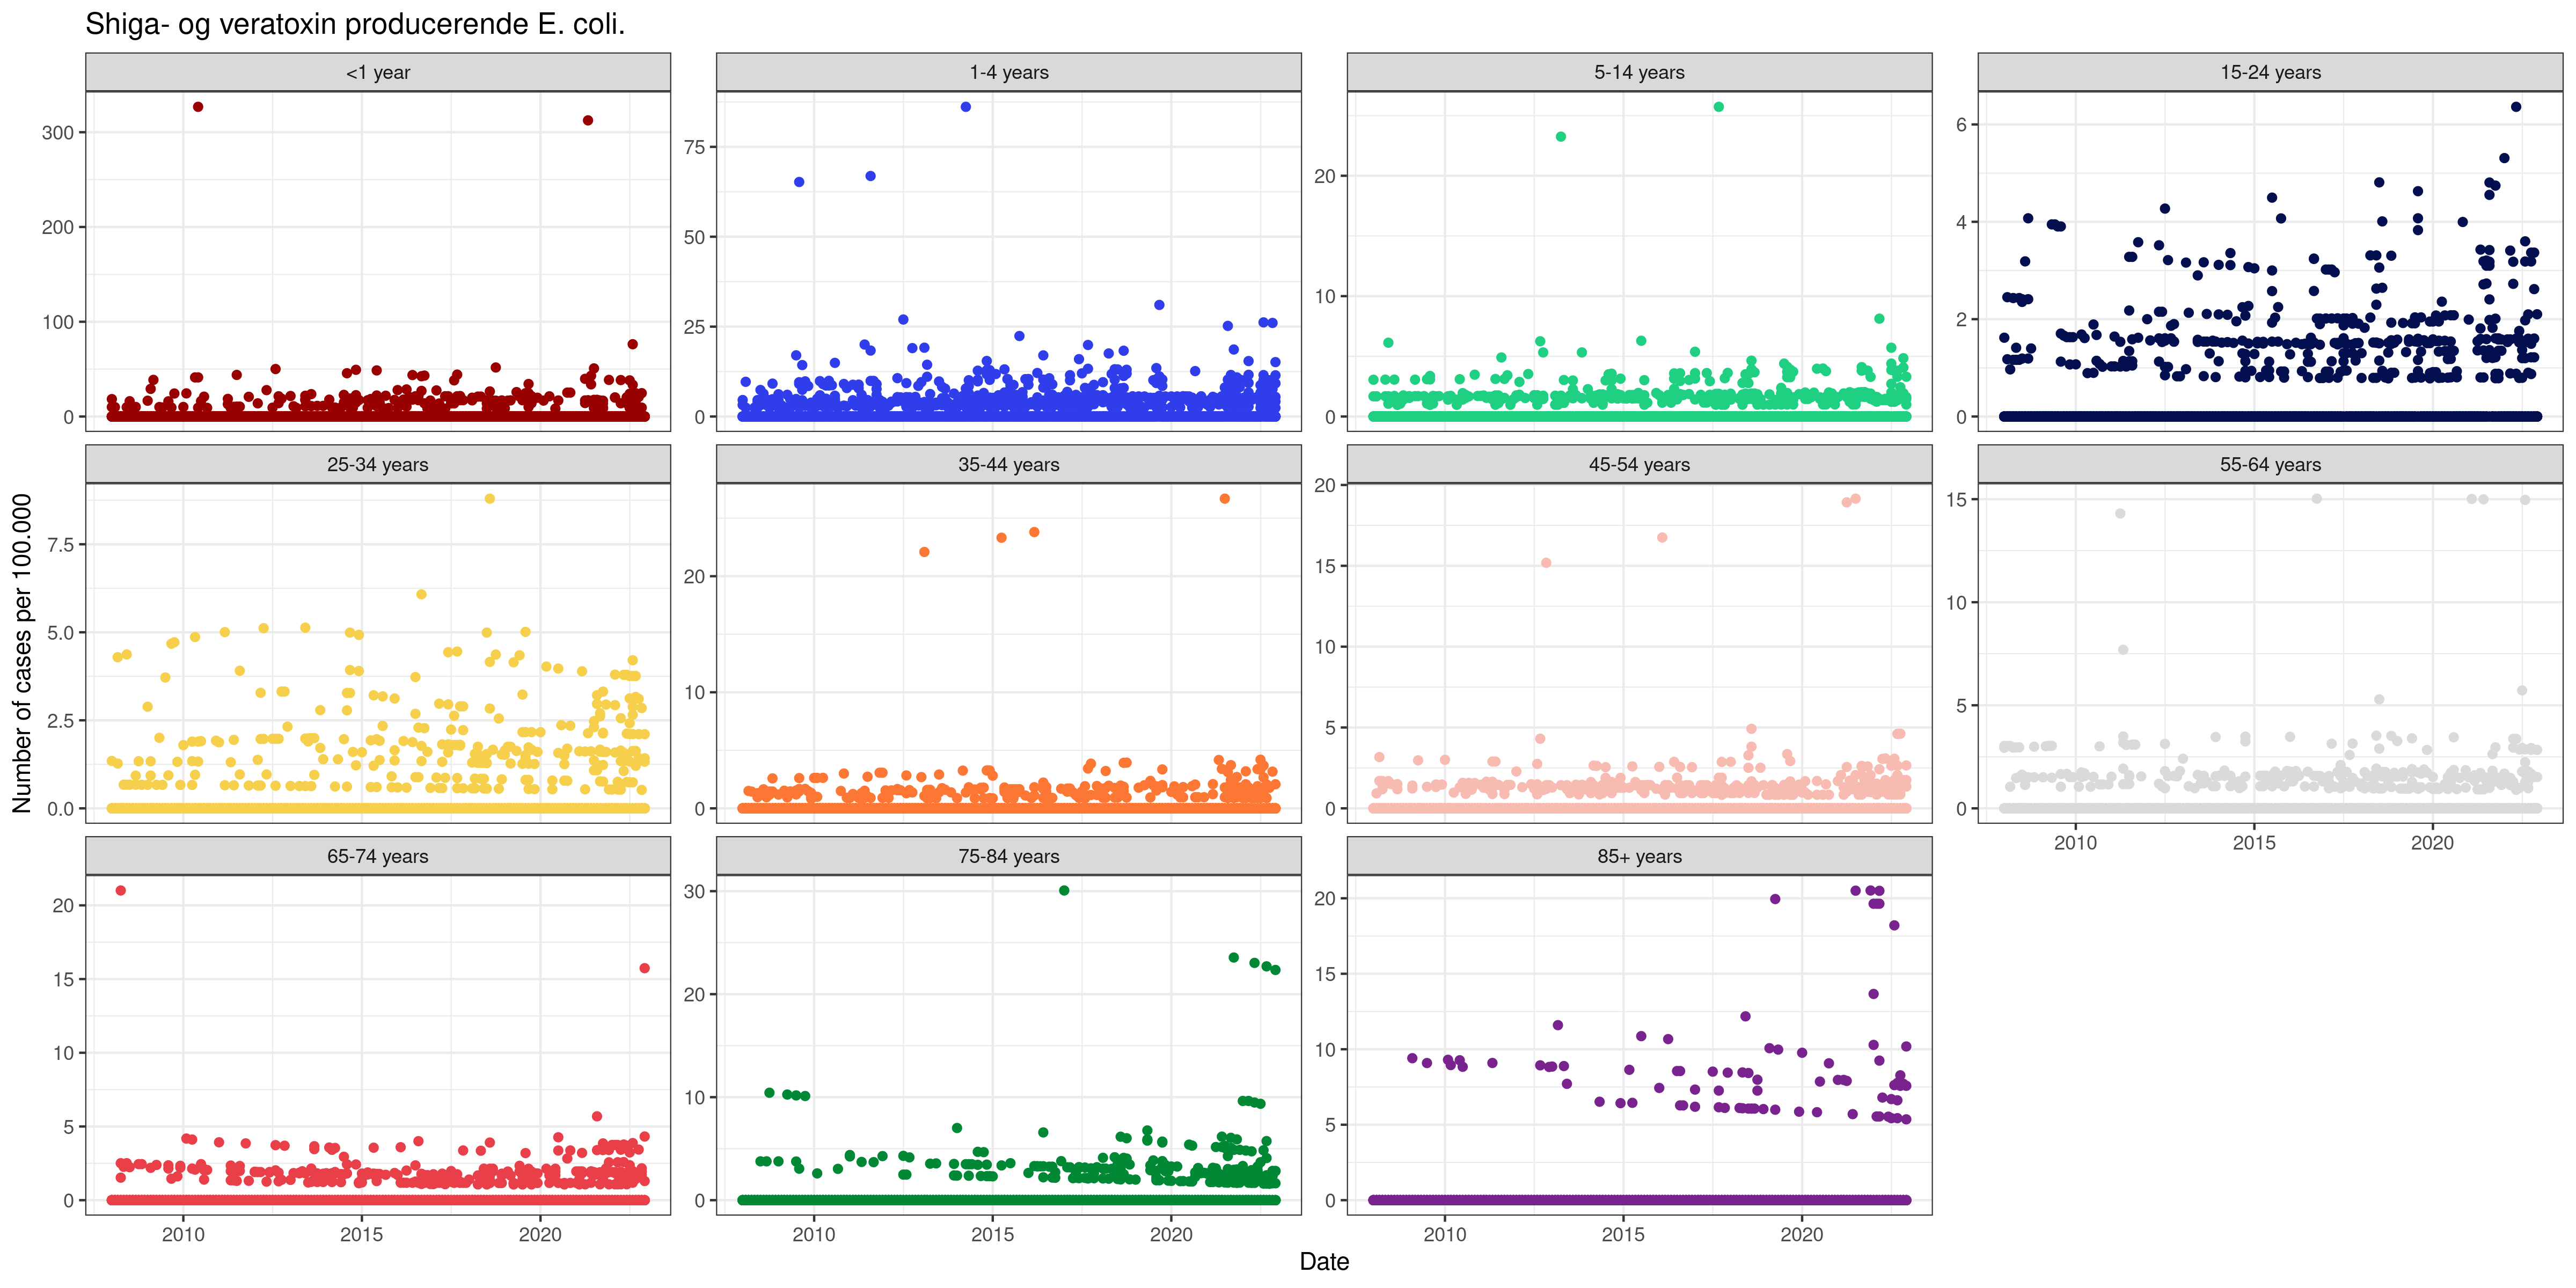
\includegraphics[width=1\linewidth]{../figures/ShigaogveratoxinproducerendeEcolixAgeGroup}

\normalsize
\end{frame}

\hypertarget{state-of-the-art-methods}{%
\section{State-of-the-art methods}\label{state-of-the-art-methods}}

\begin{frame}{State-of-the-art methods}
State-of-the-art methods for aberration detection is presented in
\cite{Salmon_2016} and implemented in the R package
\textbf{surveillance}. The R package includes methods such as the
Farrington method introduced by \cite{Farrington_1996} together with the
improvements proposed by \cite{Noufaily_2013}.
\end{frame}

\hypertarget{farrington}{%
\subsection{Farrington}\label{farrington}}

\begin{frame}{Farrington}
\tiny

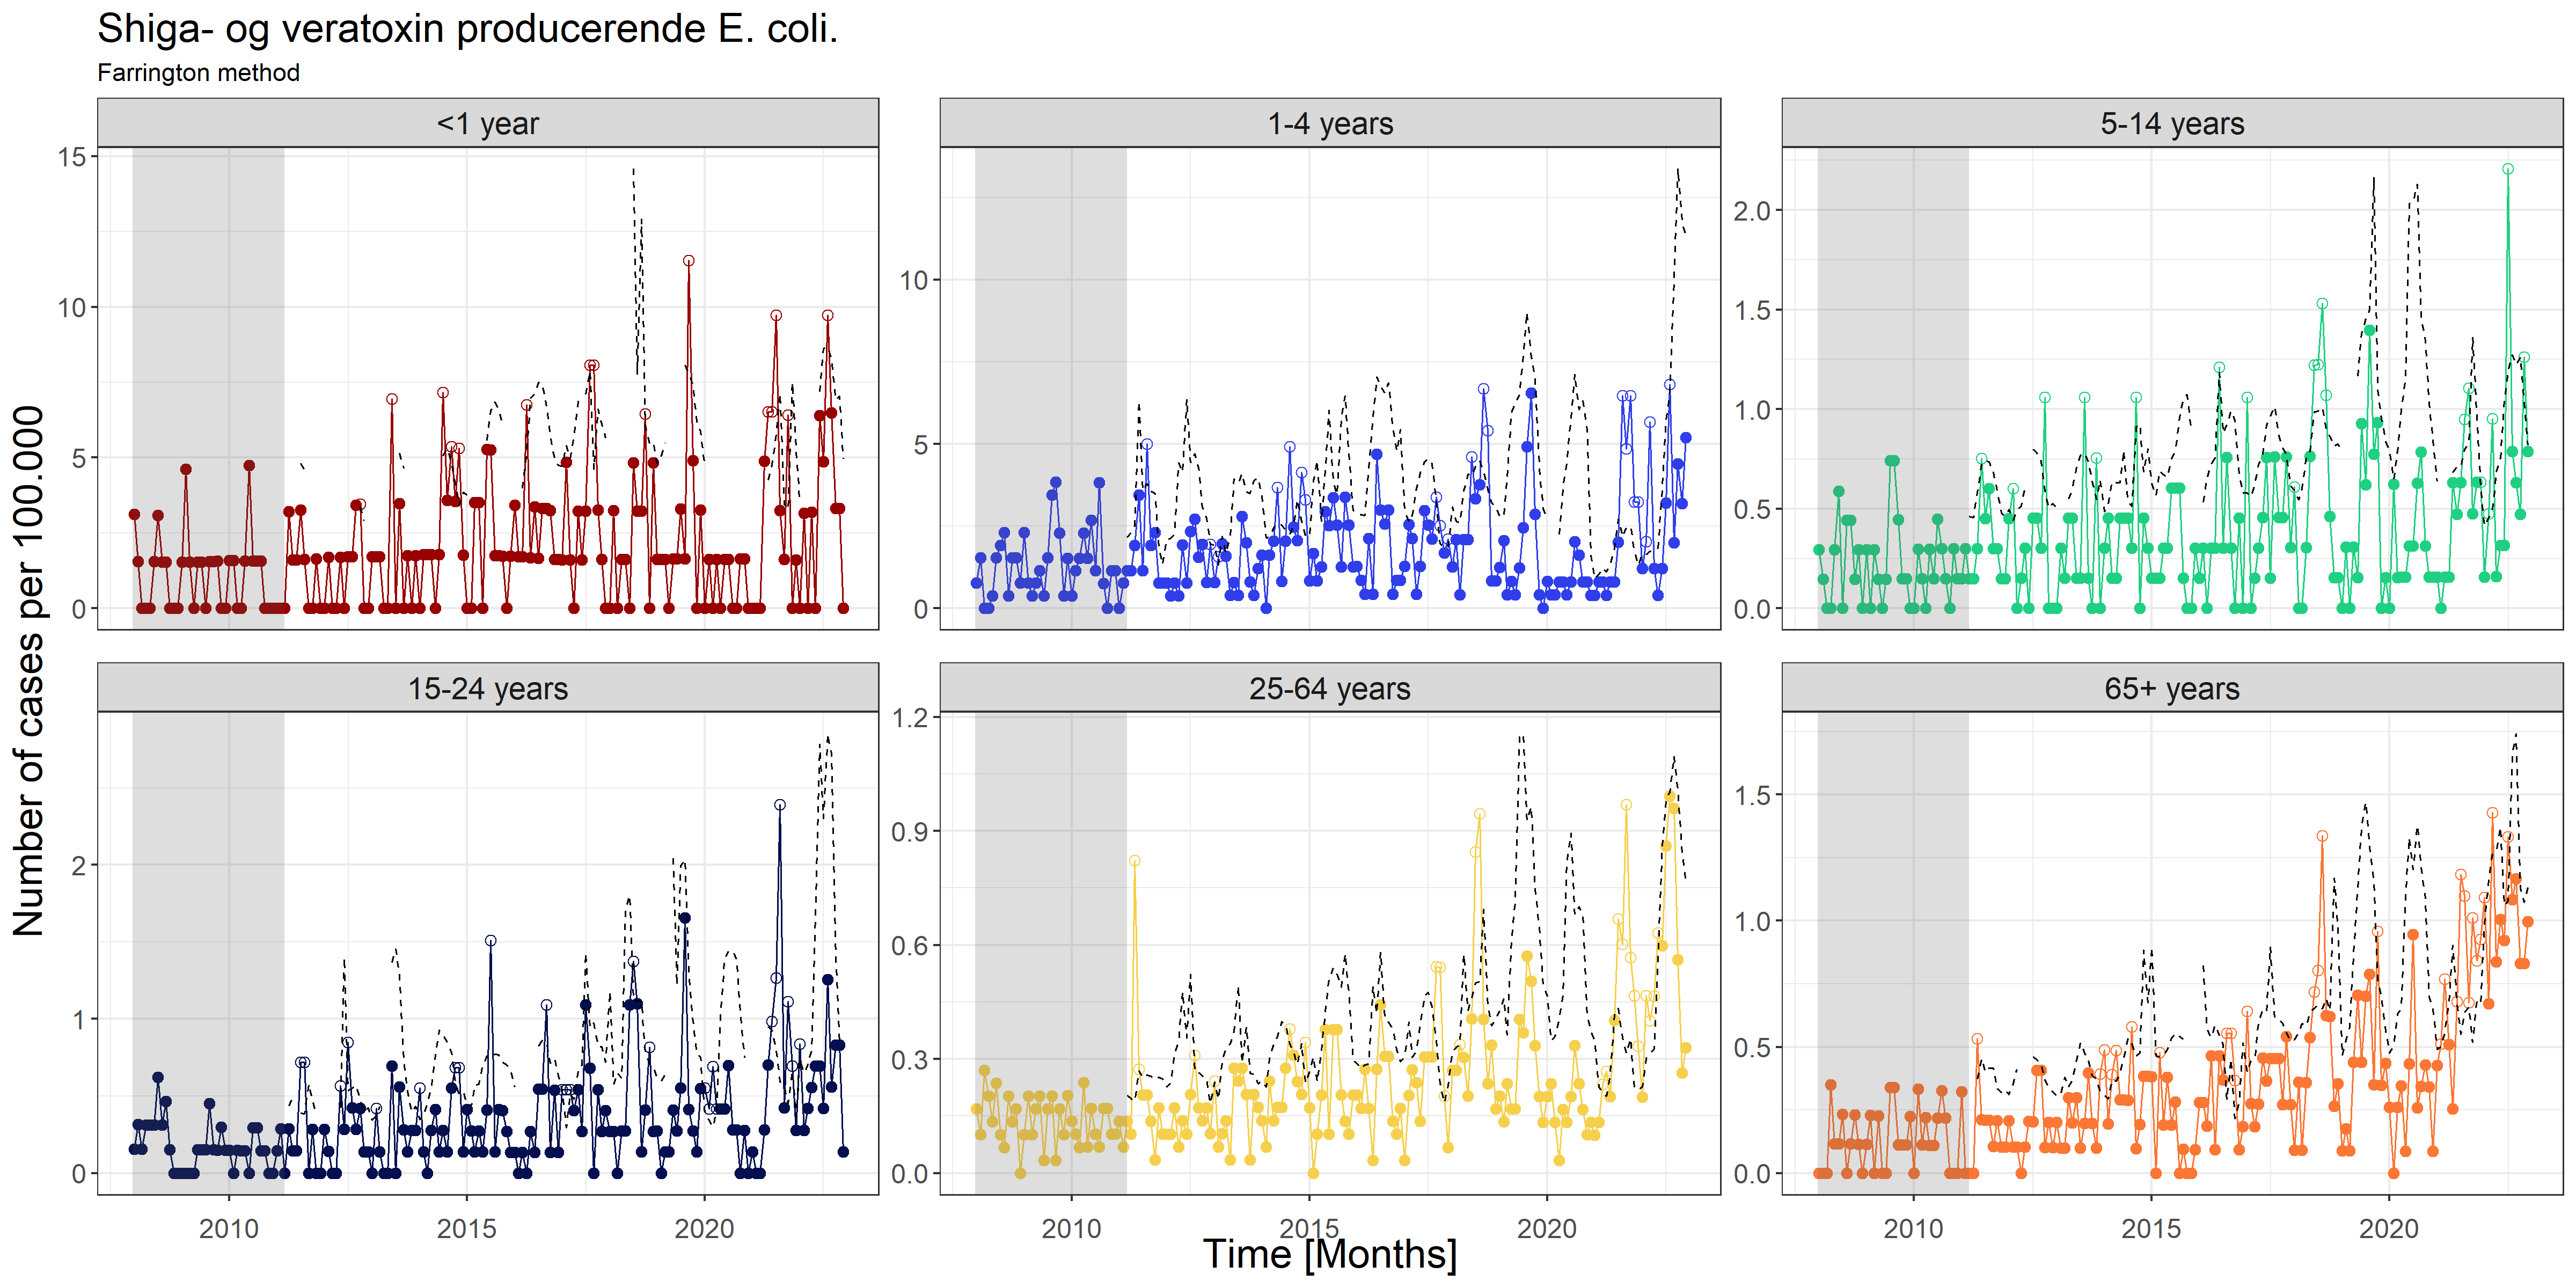
\includegraphics[width=1\linewidth]{../figures/STEC_farrington}

\normalsize
\end{frame}

\hypertarget{noufaily}{%
\subsection{Noufaily}\label{noufaily}}

\begin{frame}{Noufaily}
\tiny

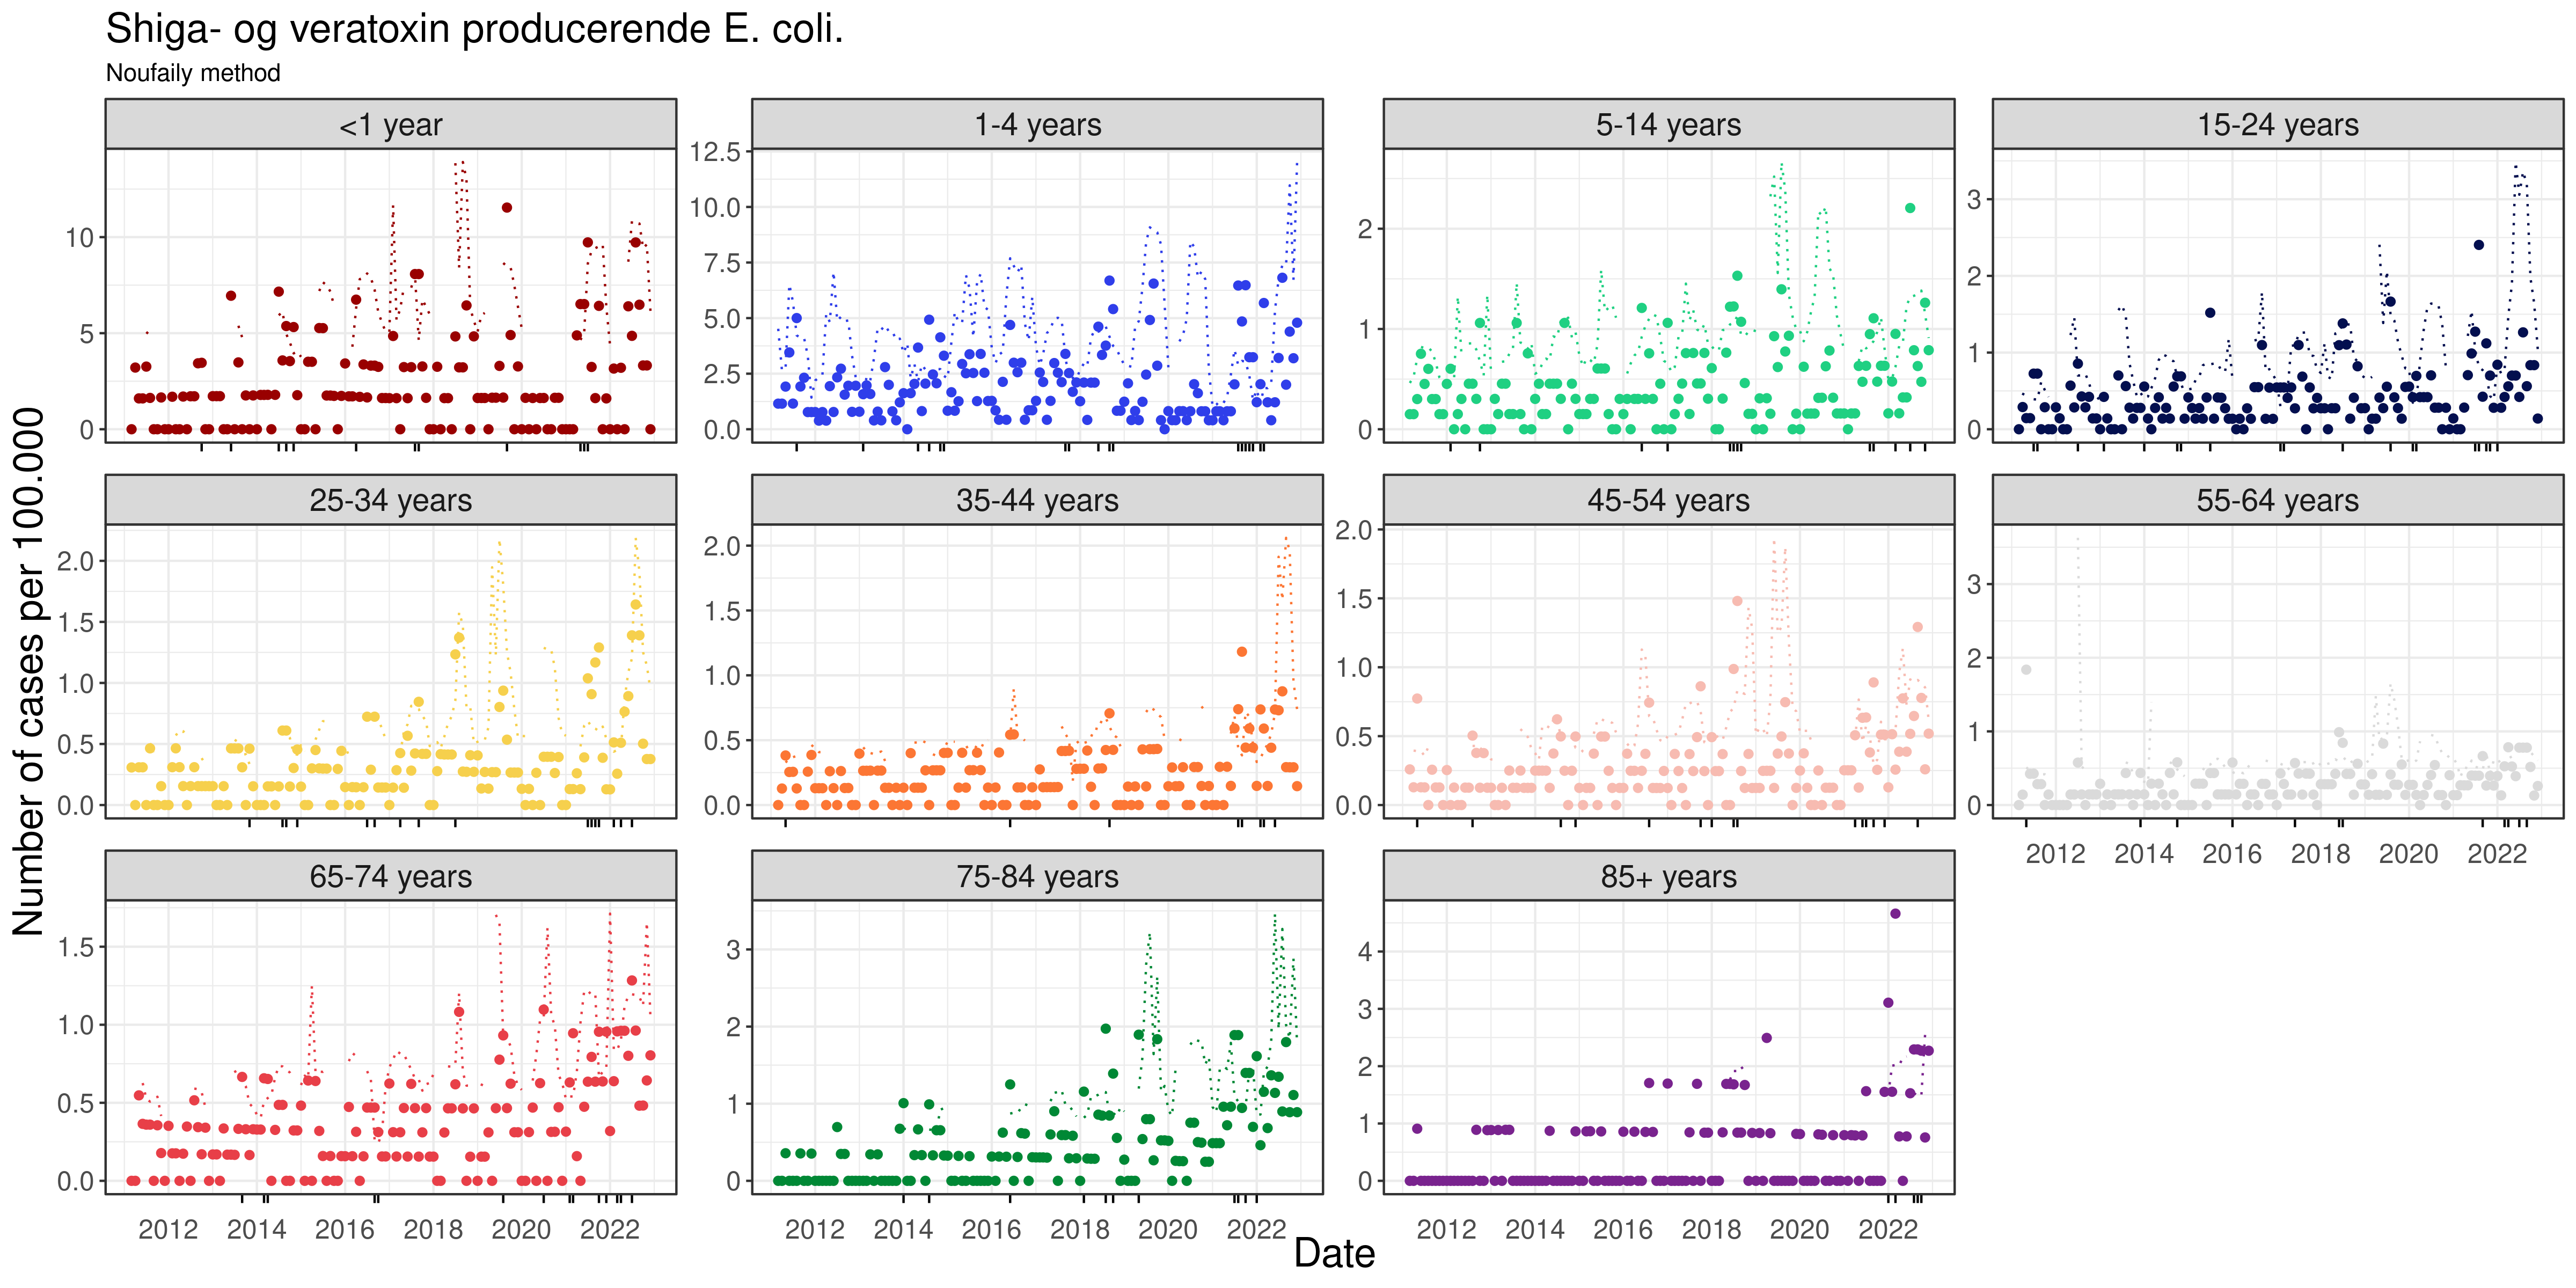
\includegraphics[width=1\linewidth]{../figures/STEC_noufaily}

\normalsize
\end{frame}

\hypertarget{novel-methods-based-on-general-mixed-effect-models}{%
\section{Novel methods based on general mixed effect
models}\label{novel-methods-based-on-general-mixed-effect-models}}

\begin{frame}{Novel methods based on general mixed effect models}
In the following two novel methods, based on theory presented in
\cite{Madsen_2010}, for aberration detection is presented. Namely, a
hierachical Poisson-Normal model and a hierachical Poisson-Gamma model.
\end{frame}

\begin{frame}{Hierachical models}
\protect\hypertarget{hierachical-models}{}
It is useful to formulate the model as a hierarchical model containing a
\textit{first stage model}

\begin{equation}
  f_{Y|u}(\boldsymbol{y};\boldsymbol{u},\boldsymbol{\beta})
\end{equation}

which is a model for the data given the random effects, and a
\textit{second stage model}

\begin{equation}
  f_U(\boldsymbol{u}, \boldsymbol{\Psi})
\end{equation}

which is a model for the random effects. The total set of parameters is
\(\boldsymbol{\theta}=(\boldsymbol{\beta}, \boldsymbol{\Psi})\).
\end{frame}

\begin{frame}{Objective}
\protect\hypertarget{objective}{}
\begin{itemize}
  \item The objective is to assess the unobserved random effects, $\boldsymbol{u}$, and determine the critical value, $C_\alpha$, with significance level $\alpha$.
  \item If $u_{it}>C_\alpha$, the observation is characterized as an outbreak.
\end{itemize}

\hfill\break
\hfill\break
\textbf{NOTE:} For this presentation a default of \(\alpha=0.05\) is
used.
\end{frame}

\hypertarget{hierachical-poisson-normal-model}{%
\subsection{Hierachical Poisson-Normal
model}\label{hierachical-poisson-normal-model}}

\begin{frame}{Hierachical Poisson-Normal model}
The model can be formulated as a two-level hierarchical model

\begin{subequations}
  \begin{alignat}{2}
    \boldsymbol{Y|u} &\sim \Pois (\boldsymbol{\lambda} e^{\boldsymbol{u}}) \label{eq:pois_ln0} \\
    \boldsymbol{u} &\sim \N (\boldsymbol{0}, \sigma^2) \label{eq:pois_ln1}
  \end{alignat}
\end{subequations}
\end{frame}

\begin{frame}{Hierachical Poisson-Normal model}
\protect\hypertarget{hierachical-poisson-normal-model-1}{}
\begin{itemize}
  \item $\boldsymbol{Y|u}$ are assumed to be a Poisson distribution with intensities $\boldsymbol{\lambda}$.
  \item An offset is included to account for the population size, $x_{it}$.
  \item Hence, the model for the fixed effect is
\end{itemize}

\begin{equation}
  \log(\lambda_{i})=\boldsymbol{X}_i^T\boldsymbol{\beta}+\log(x_{it})
\end{equation}

\begin{itemize}
  \item Here $\boldsymbol{X}_i$ is a $p$-dimensional vector of covariates, and $\boldsymbol{\beta}$ contains the corresponding fixed effect parameters.
  \item The random effects $\boldsymbol{u}$ are assumed to be Gaussian.
\end{itemize}

\begin{equation}
  u_{it} = \epsilon_{it}
\end{equation}

\begin{itemize}
  \item Here $\epsilon_{it}\sim\N(\boldsymbol{0},\sigma^2)$ is a white noise process, and $\sigma$ is a model parameter.
  \item The model parameters are estimated in a rolling window of length \textit{k}.
\end{itemize}
\end{frame}

\begin{frame}{Results}
\protect\hypertarget{results}{}
\tiny

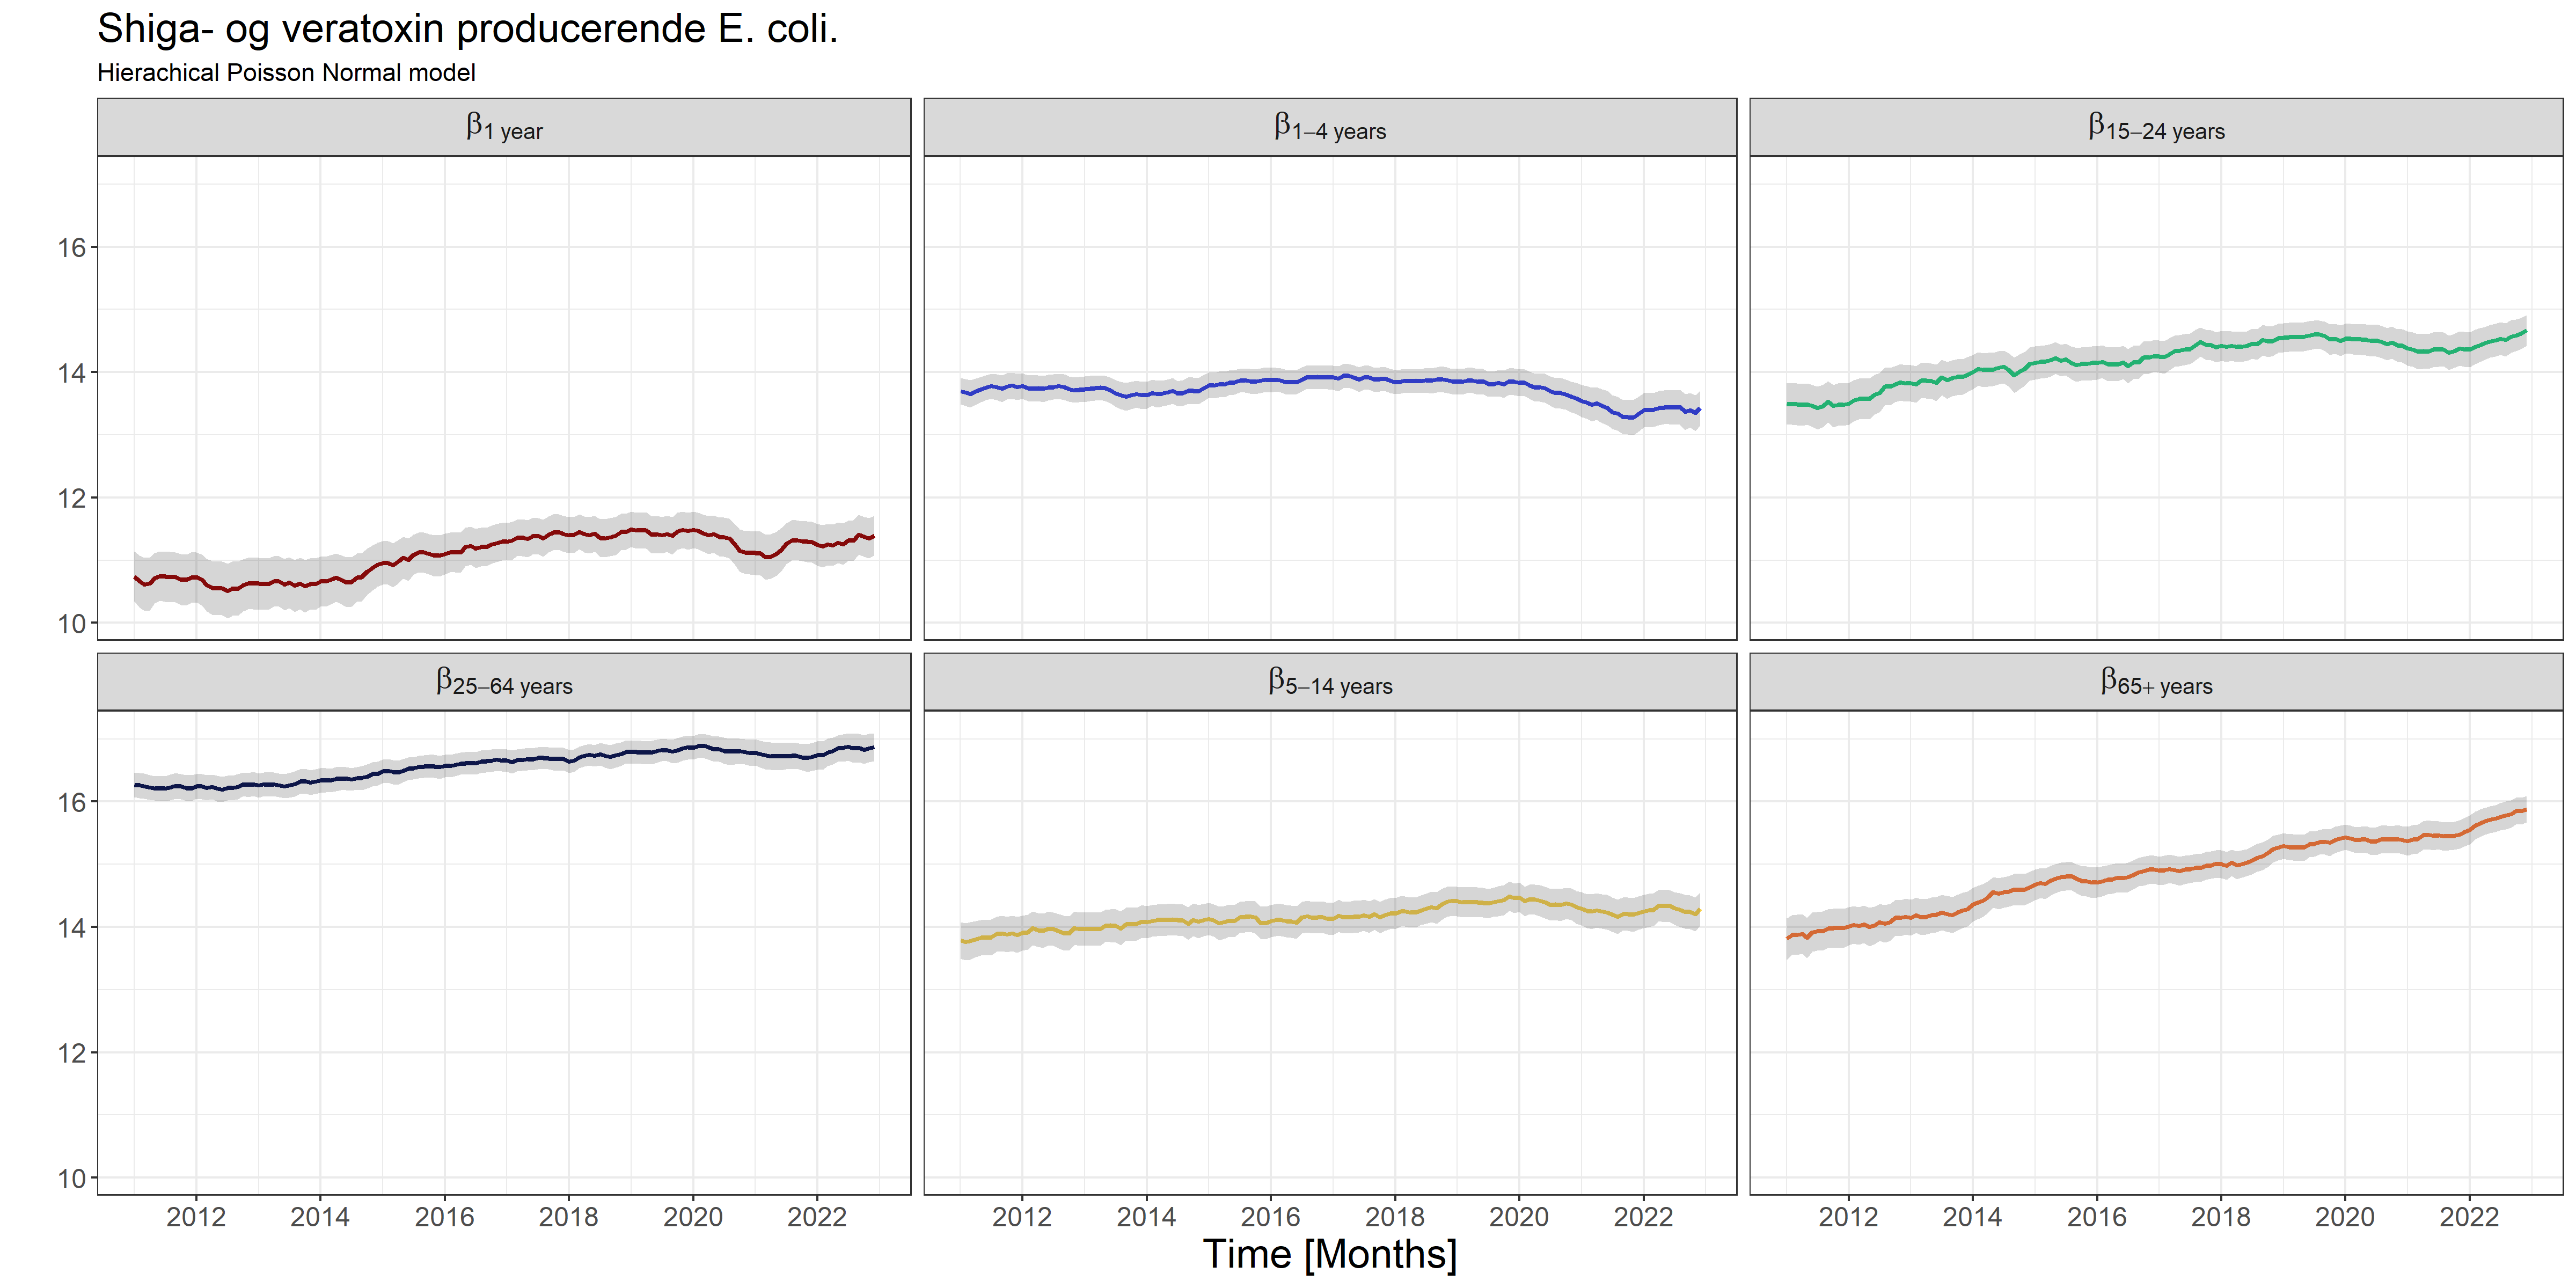
\includegraphics[width=1\linewidth]{../figures/thetaSTECPoisNExclude}

\normalsize
\end{frame}

\begin{frame}{Results}
\protect\hypertarget{results-1}{}
\tiny

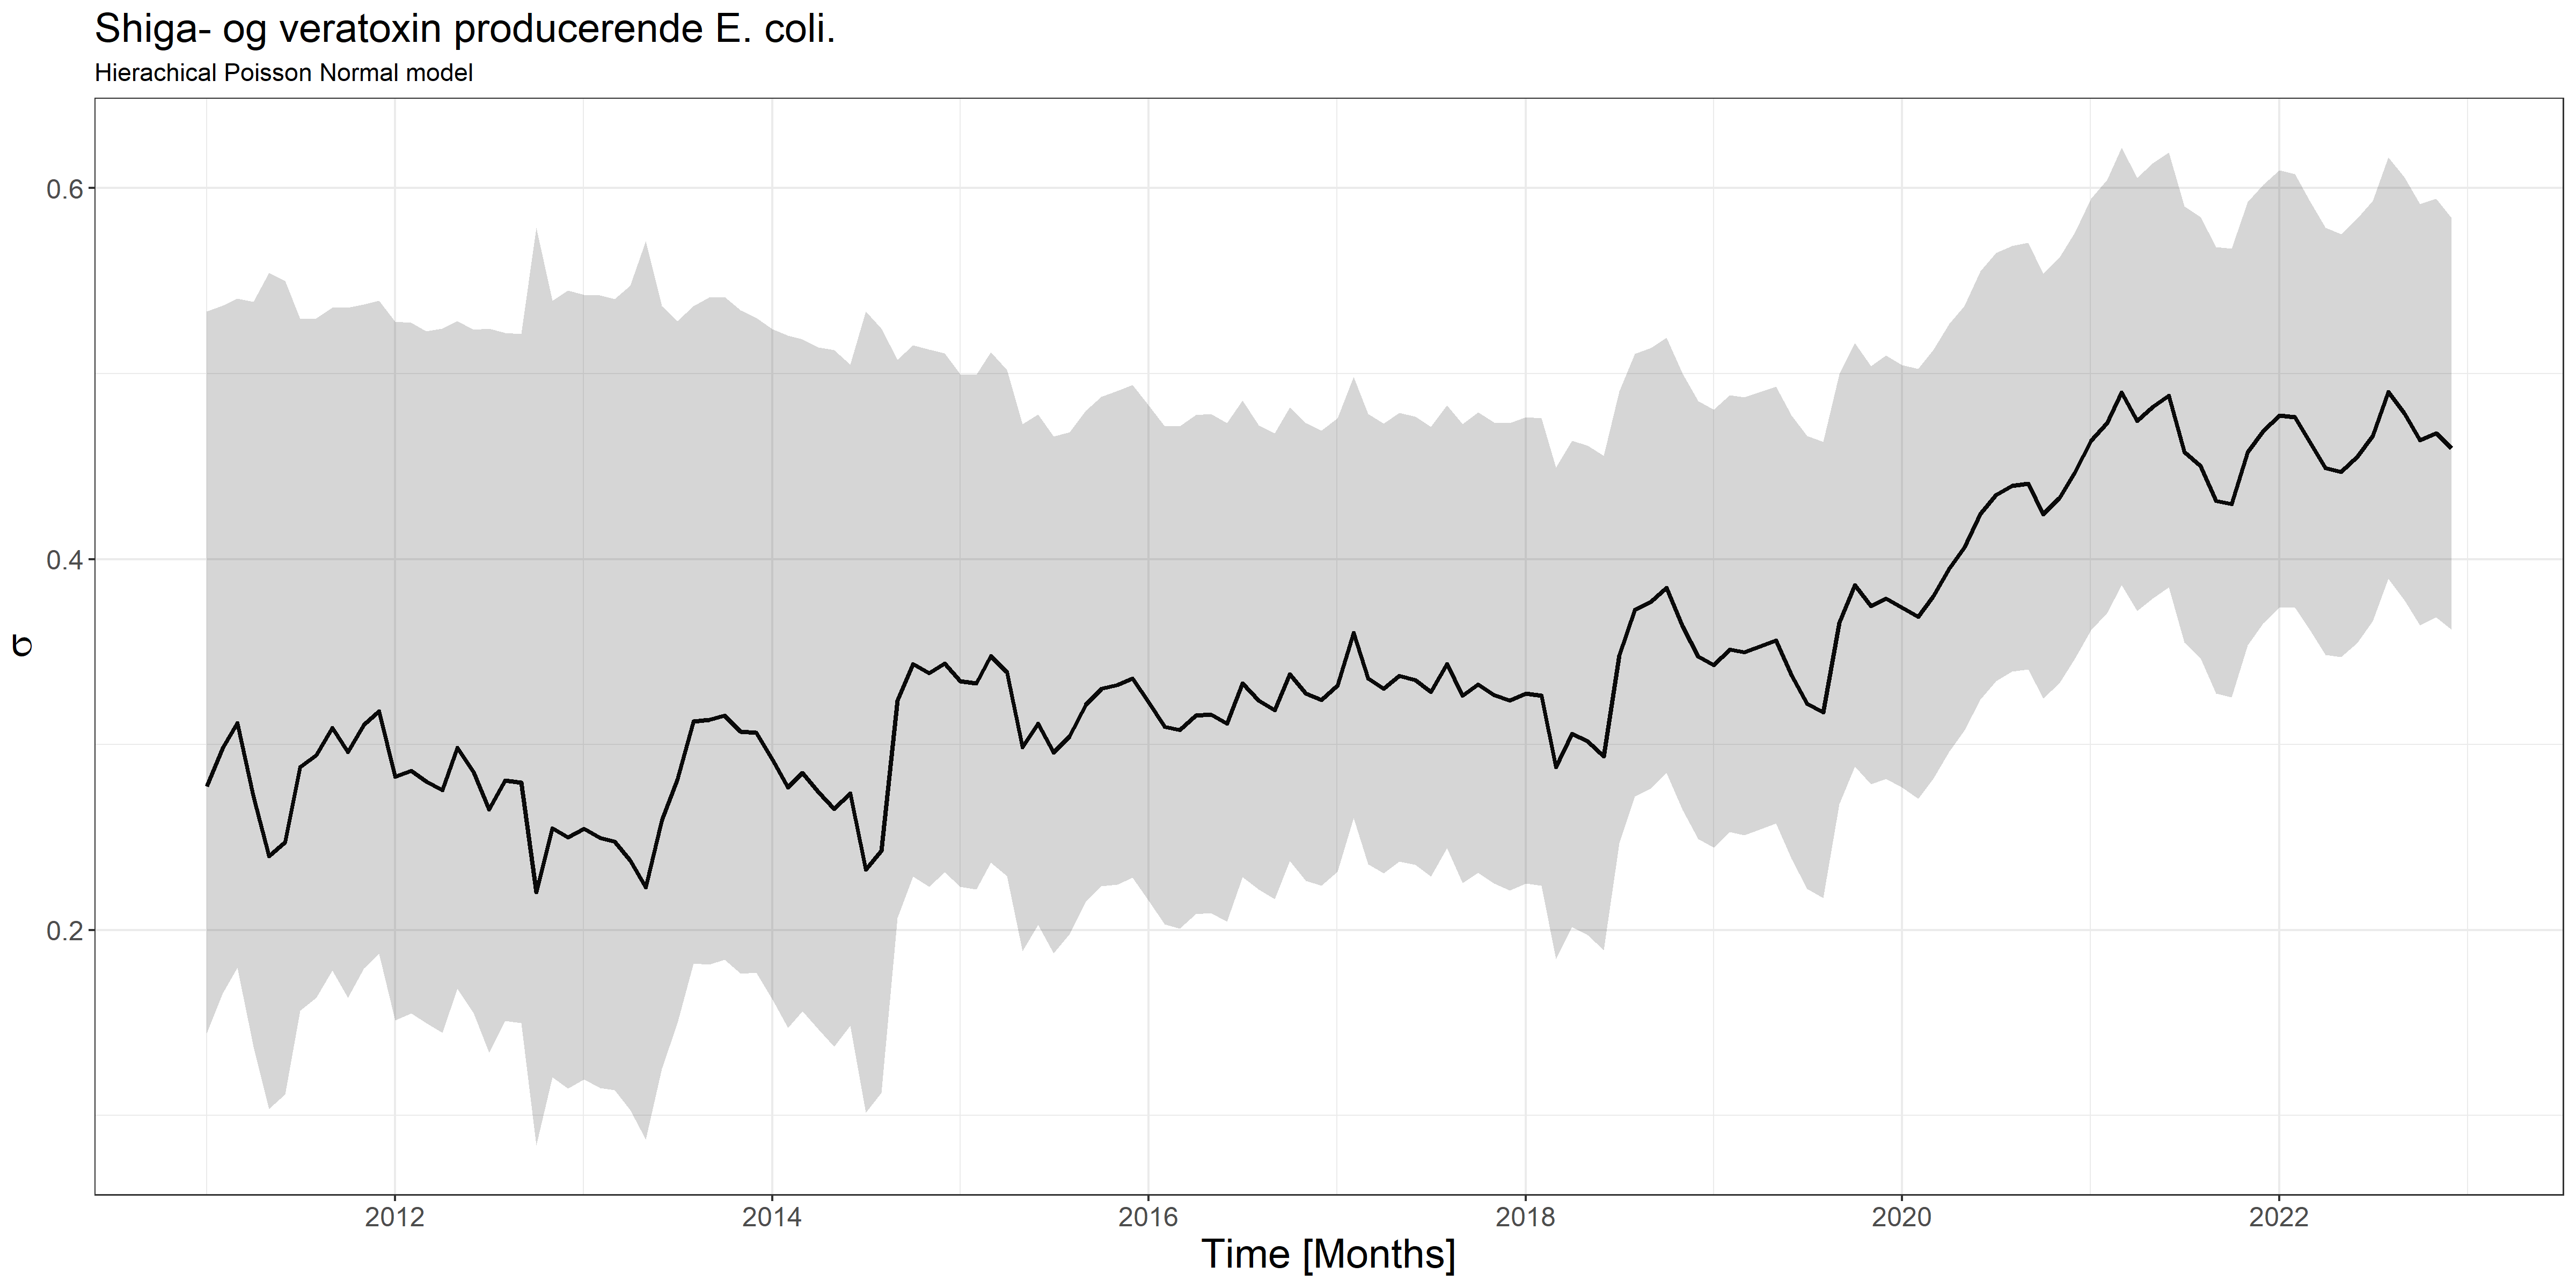
\includegraphics[width=1\linewidth]{../figures/phiSTECPoisNExclude}

\normalsize
\end{frame}

\begin{frame}{Threshold calculation}
\protect\hypertarget{threshold-calculation}{}
The critical value, \(C_\alpha\), is computed from the
\(1-\alpha\)-quantile of the Normal distribution with the
maximum-likelihood estimate for the variance, \(\hat\sigma\).

\begin{equation}
  C_\alpha=\N(\boldsymbol{0},\hat\sigma^2)_{1-\alpha}
\end{equation}
\end{frame}

\begin{frame}{Results - Out-of-sample random effects}
\protect\hypertarget{results---out-of-sample-random-effects}{}
\tiny

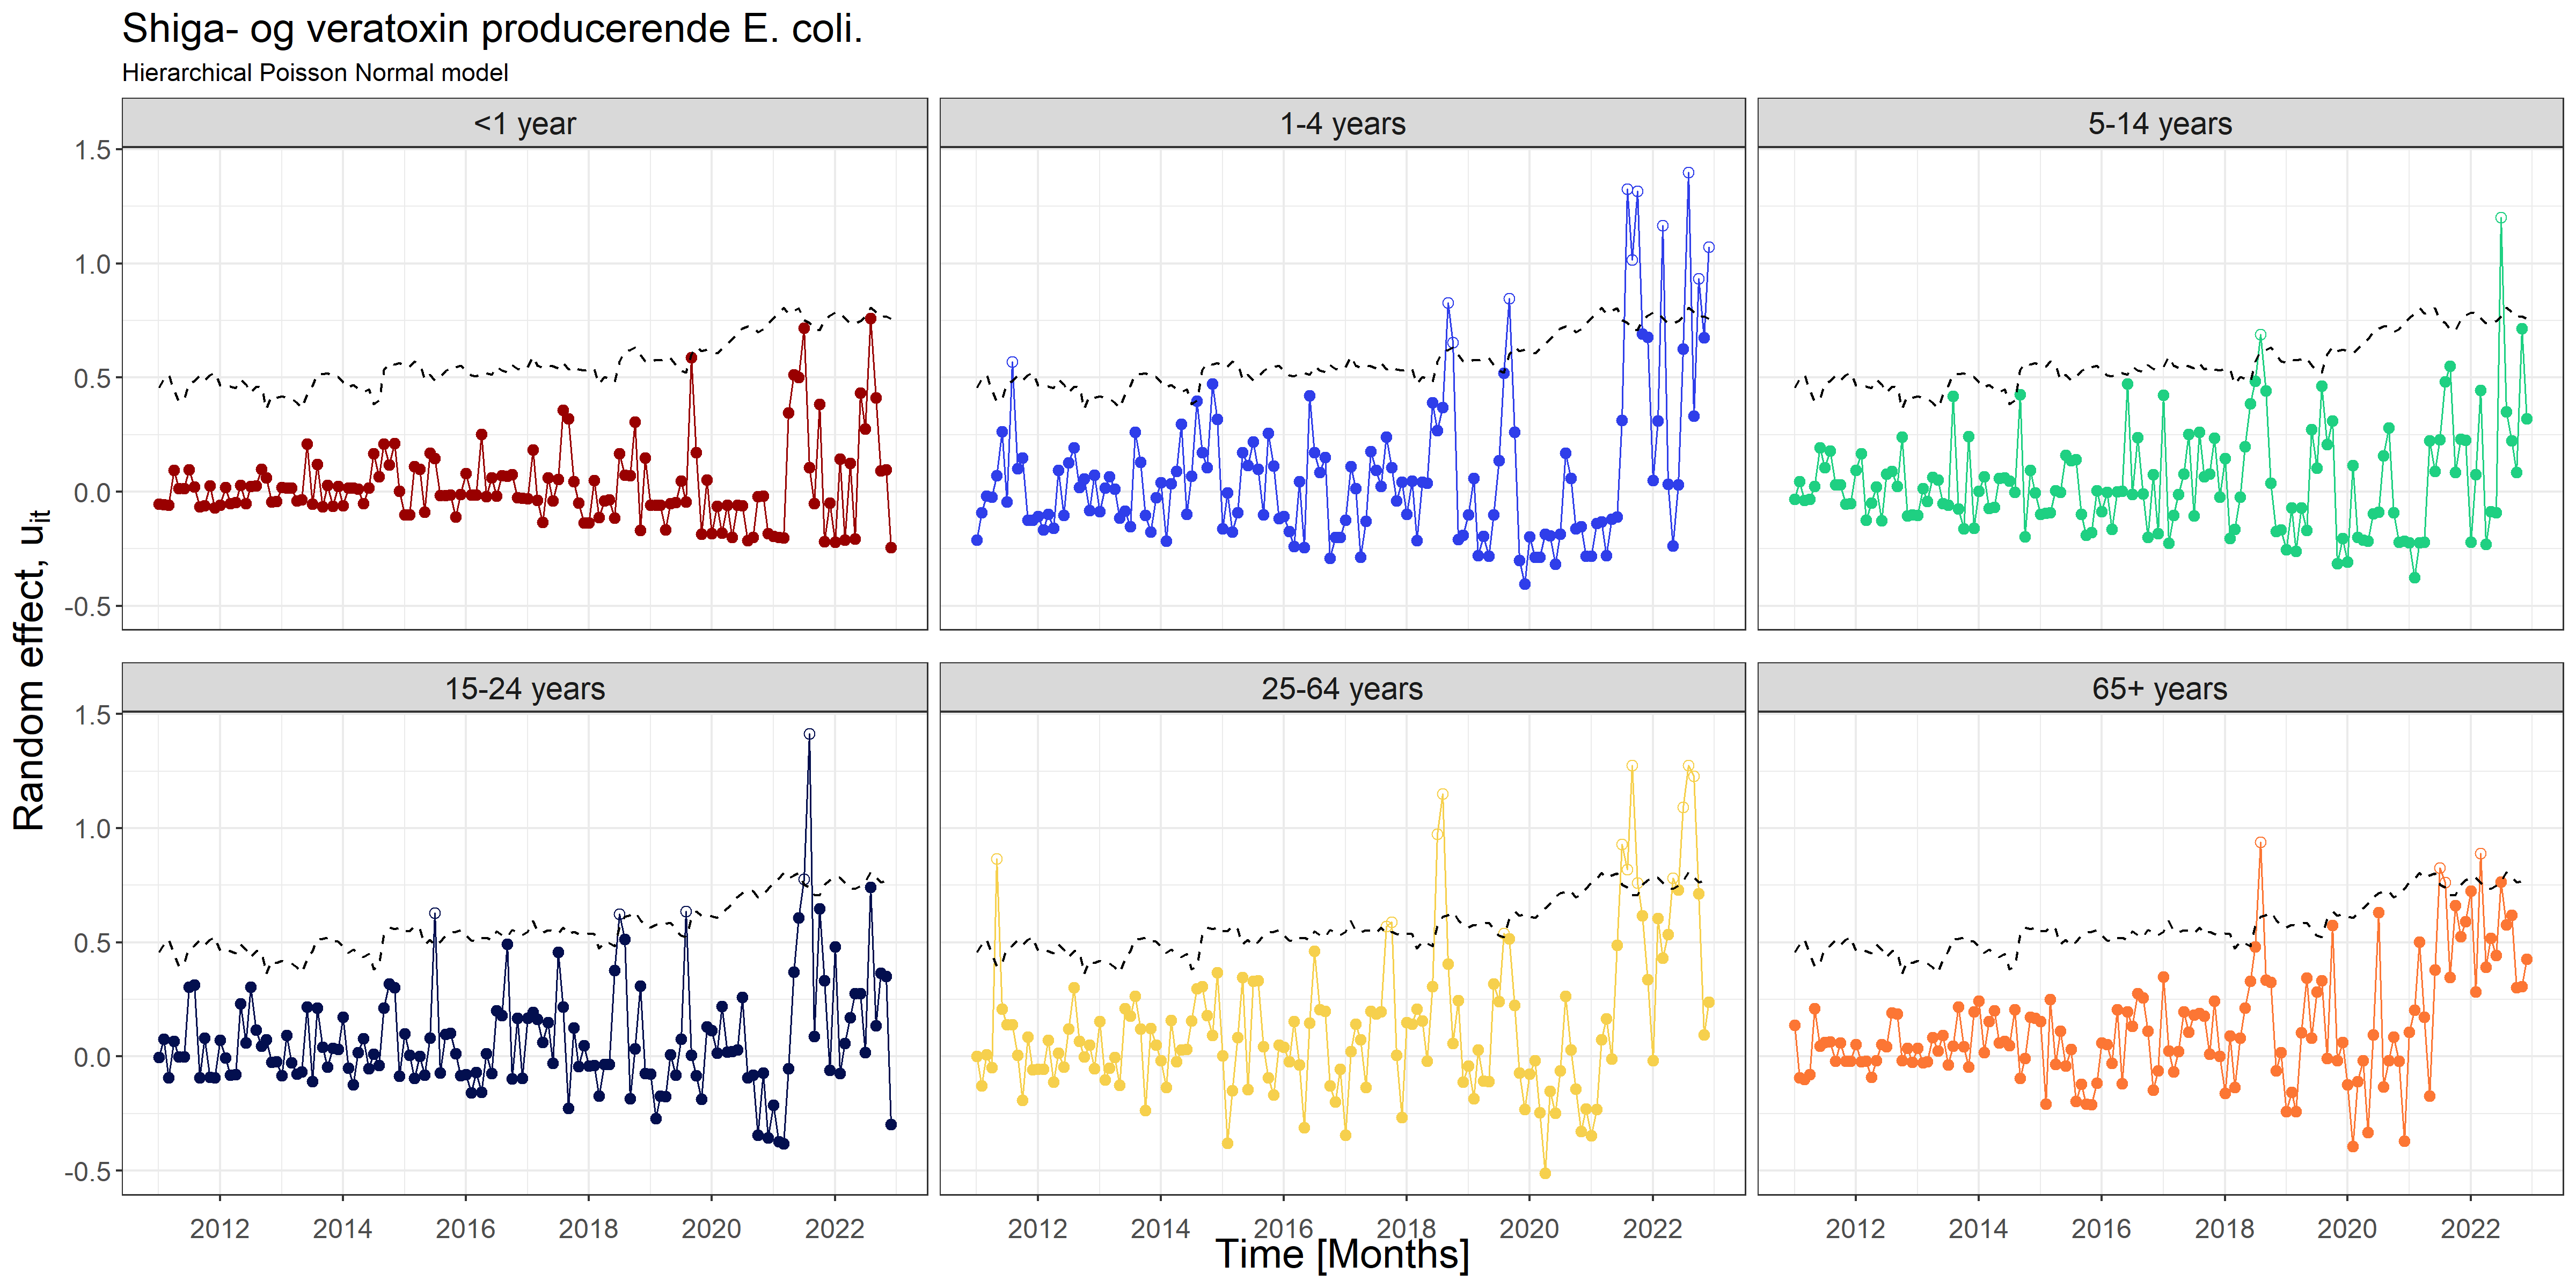
\includegraphics[width=1\linewidth]{../figures/windowedSTEDPoisNExclude}

\normalsize
\end{frame}

\hypertarget{hierachical-poisson-gamma-model}{%
\subsection{Hierachical Poisson-Gamma
model}\label{hierachical-poisson-gamma-model}}

\begin{frame}{Hierachical Poisson-Gamma model}
\begin{itemize}
  \item $\boldsymbol{Y|u}$ are assumed to follow a Poisson distribution. 
  \item The intensities, $\lambda_{i}$, are defined as
\end{itemize}

\begin{equation}
  \log(\lambda_{i})=\boldsymbol{X}_{i}^{T}\boldsymbol{\beta}+\log(x_{it})
\end{equation}

\begin{itemize}
  \item Here $\boldsymbol{X}_{i}$ is a $p$-dimensional vector of covariates, and $\boldsymbol{\beta}$ contains the corresponding fixed effect parameter.
  \item The random effects $\boldsymbol{u}$ are assumed to follow a reparametrized Gamma distribution with mean $\boldsymbol{1}$.
  \item The model parameters are estimated in a rolling window of length \textit{k}.
\end{itemize}
\end{frame}

\begin{frame}{Hierachical Poisson-Gamma model}
\protect\hypertarget{hierachical-poisson-gamma-model-1}{}
Subsequently, the model can be formulated as a two-level hierarchical
model

\begin{subequations} \label{eq:PoisGam}
  \begin{alignat}{2}
    \boldsymbol{Y|u} &\sim \Pois (\boldsymbol{\lambda} \boldsymbol{u}) \label{eq:pois_g0} \\ 
    \boldsymbol{u} &\sim \G(\boldsymbol{1}/\phi,\phi) \label{eq:pois_g1}
  \end{alignat}
\end{subequations}
\end{frame}

\begin{frame}{Probability function for \(Y\)}
\protect\hypertarget{probability-function-for-y}{}
\begin{equation} \label{eq:pdfMix}
  \begin{aligned}
    P[Y=y_i]&=g_{Y}(y;\lambda, \phi) \\
    &=\frac{\lambda^{y}}{y!\Gamma(1/\phi)\phi^{1/\phi}}\frac{\phi^{y+1/\phi}\Gamma(y+1/\phi)}{(\lambda \phi + 1)^{y+1/\phi}} \\
    &=\frac{\Gamma(y+1/\phi)}{\Gamma(1/\phi)y!}\frac{1}{(\lambda\phi+1)^{1/\phi}}\bigg(\frac{\lambda\phi}{\lambda\phi+1}\bigg)^{y} \\
    &=\begin{pmatrix} y+1/\phi-1 \\ y \end{pmatrix} \frac{1}{(\lambda\phi+1)^{1/\phi}}\bigg(\frac{\lambda\phi}{\lambda\phi+1}\bigg)^{y} \ , \ for \ y = 0, 1, 2, \dots
  \end{aligned}
\end{equation}

where we have used the convention

\begin{equation}
  \begin{pmatrix} z\\y \end{pmatrix} = \frac{\Gamma(z+1)}{\Gamma(z+1-y)y!}
\end{equation}

The marginal distribution of \(Y\) is a negative binomial distribution,
\(Y\sim \NB\big(1/\phi,1/(\lambda \phi+1)\big)\)
\end{frame}

\begin{frame}{Inference on individual group means}
\protect\hypertarget{inference-on-individual-group-means}{}
Consider the hierarchical Poisson-Gamma model in \eqref{eq:PoisGam}, and
assume that a value \(Y=y\) has been observed. Then the conditional
distribution of \(u\) for given \(Y=y\) is a Gamma distribution,

\begin{equation}
  u|Y=y\sim \G\big(y+1/\phi,\phi/(\lambda \phi+1)\big)
\end{equation}

with mean

\begin{equation}
  \E[u|Y=y]=\frac{y\phi+1}{\lambda\phi+1}
\end{equation}

and variance

\begin{equation}
  \V[u|Y=y]=\frac{(y \phi^2+\phi)}{(\lambda \phi + 1)^2}
\end{equation}
\end{frame}

\begin{frame}{Results}
\protect\hypertarget{results-2}{}
\tiny

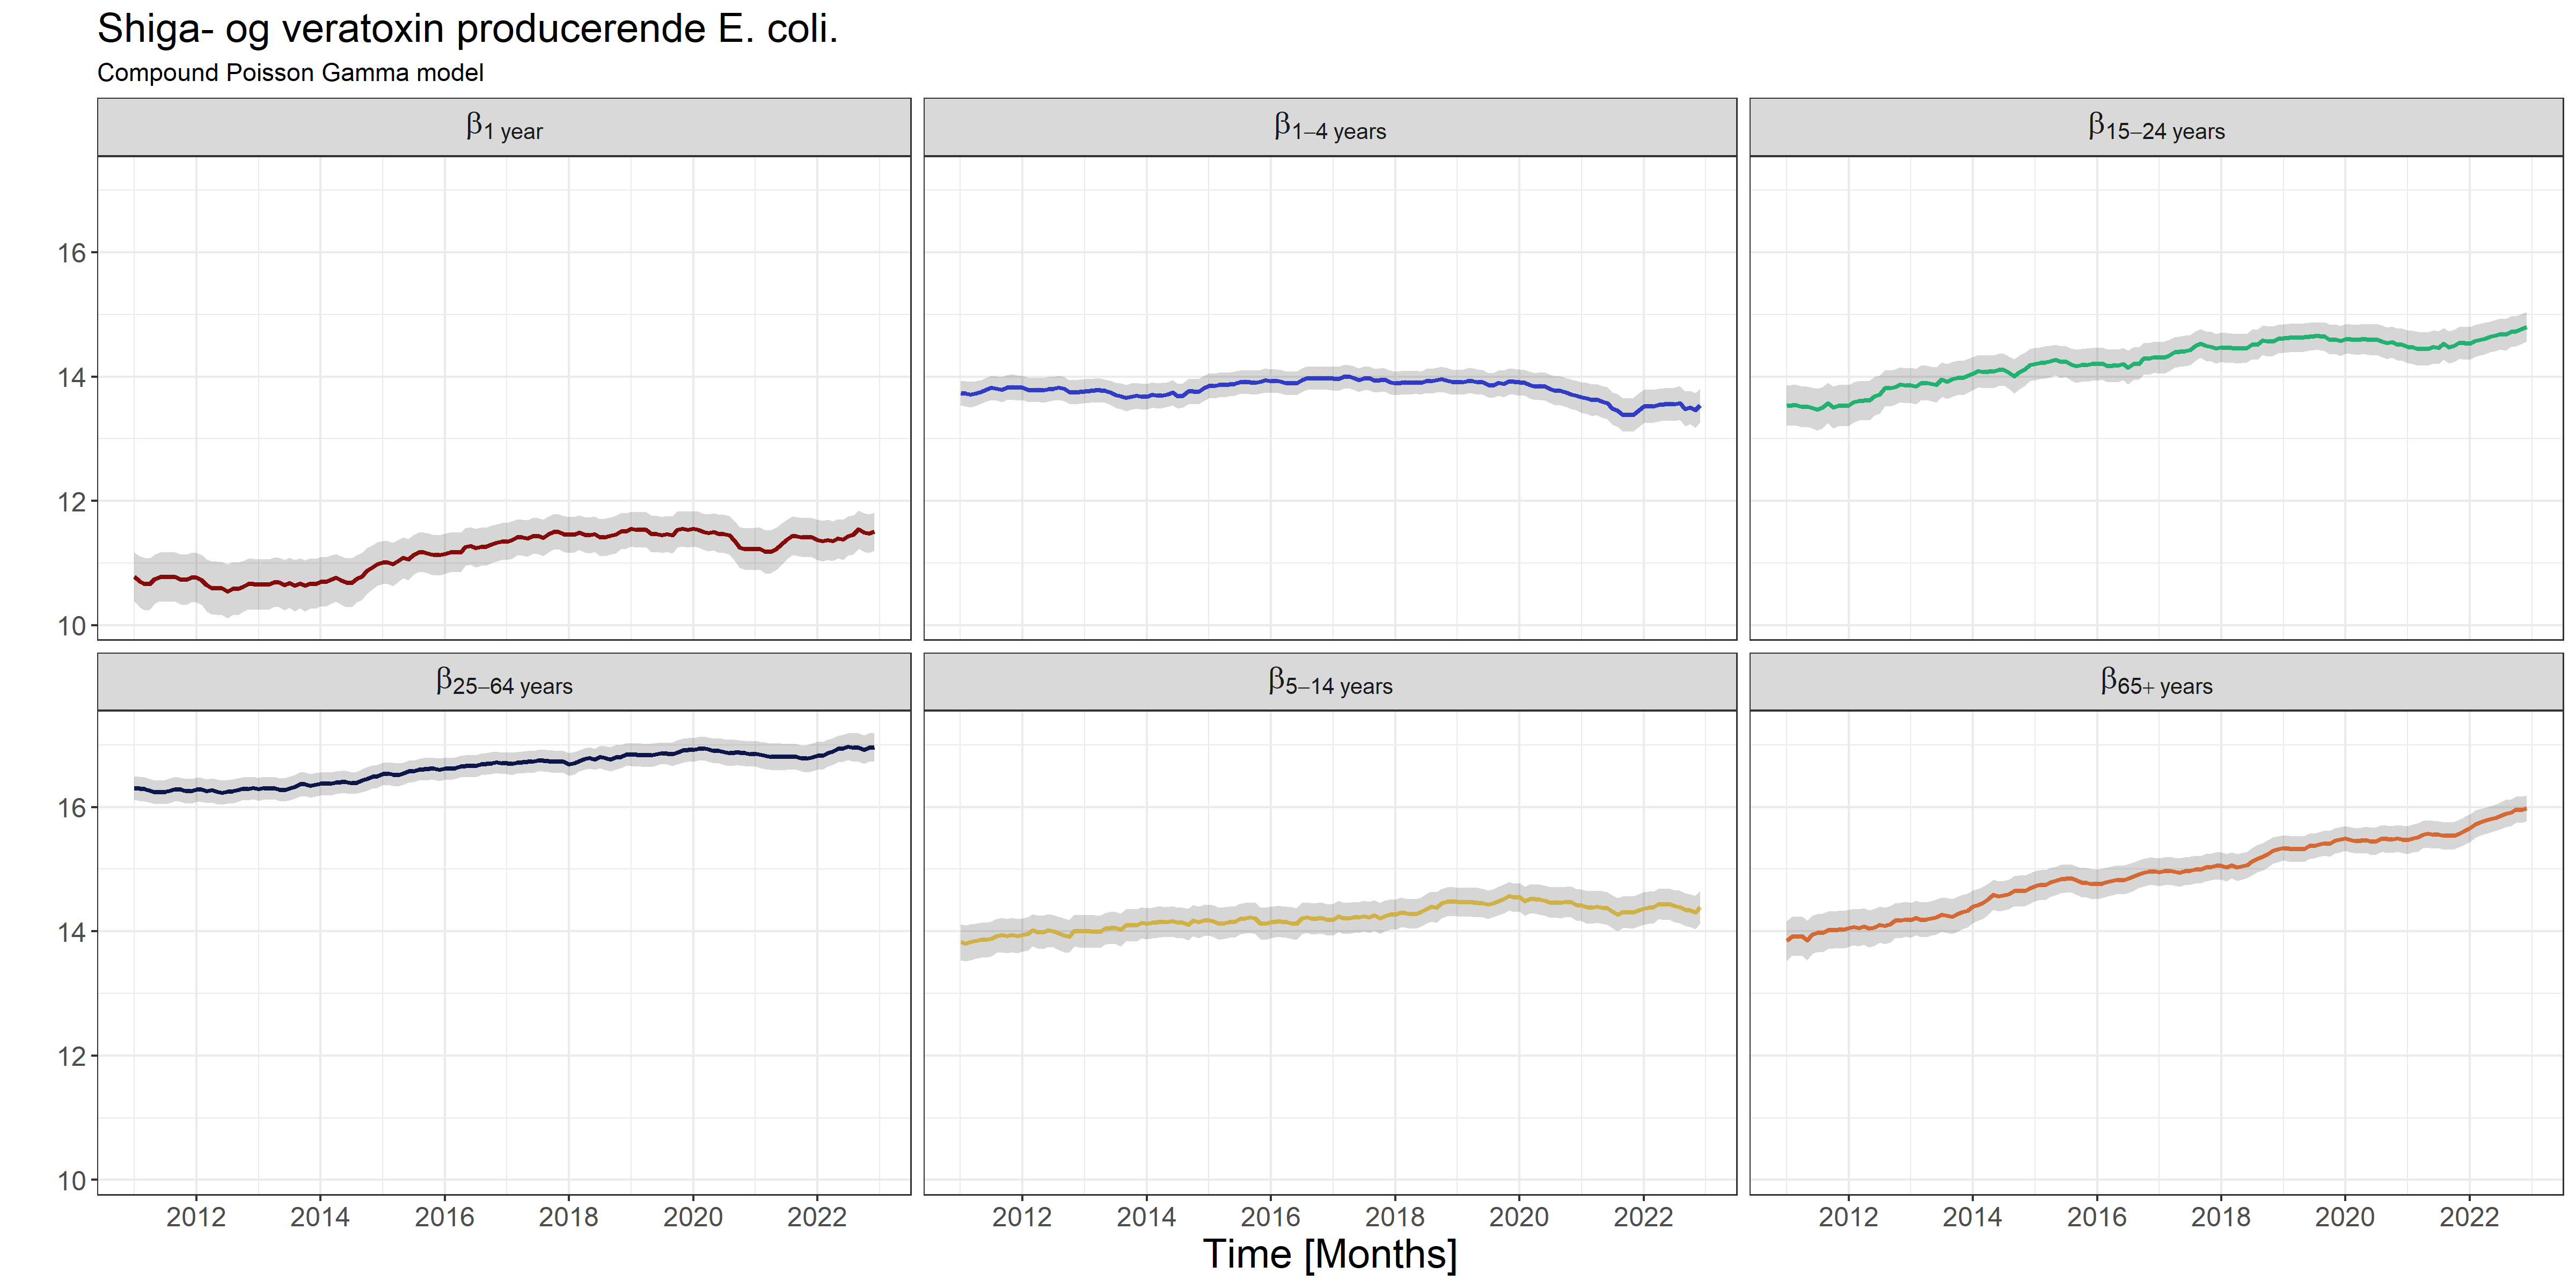
\includegraphics[width=1\linewidth]{../figures/thetaSTECPoisGExclude}

\normalsize
\end{frame}

\begin{frame}{Results}
\protect\hypertarget{results-3}{}
\tiny

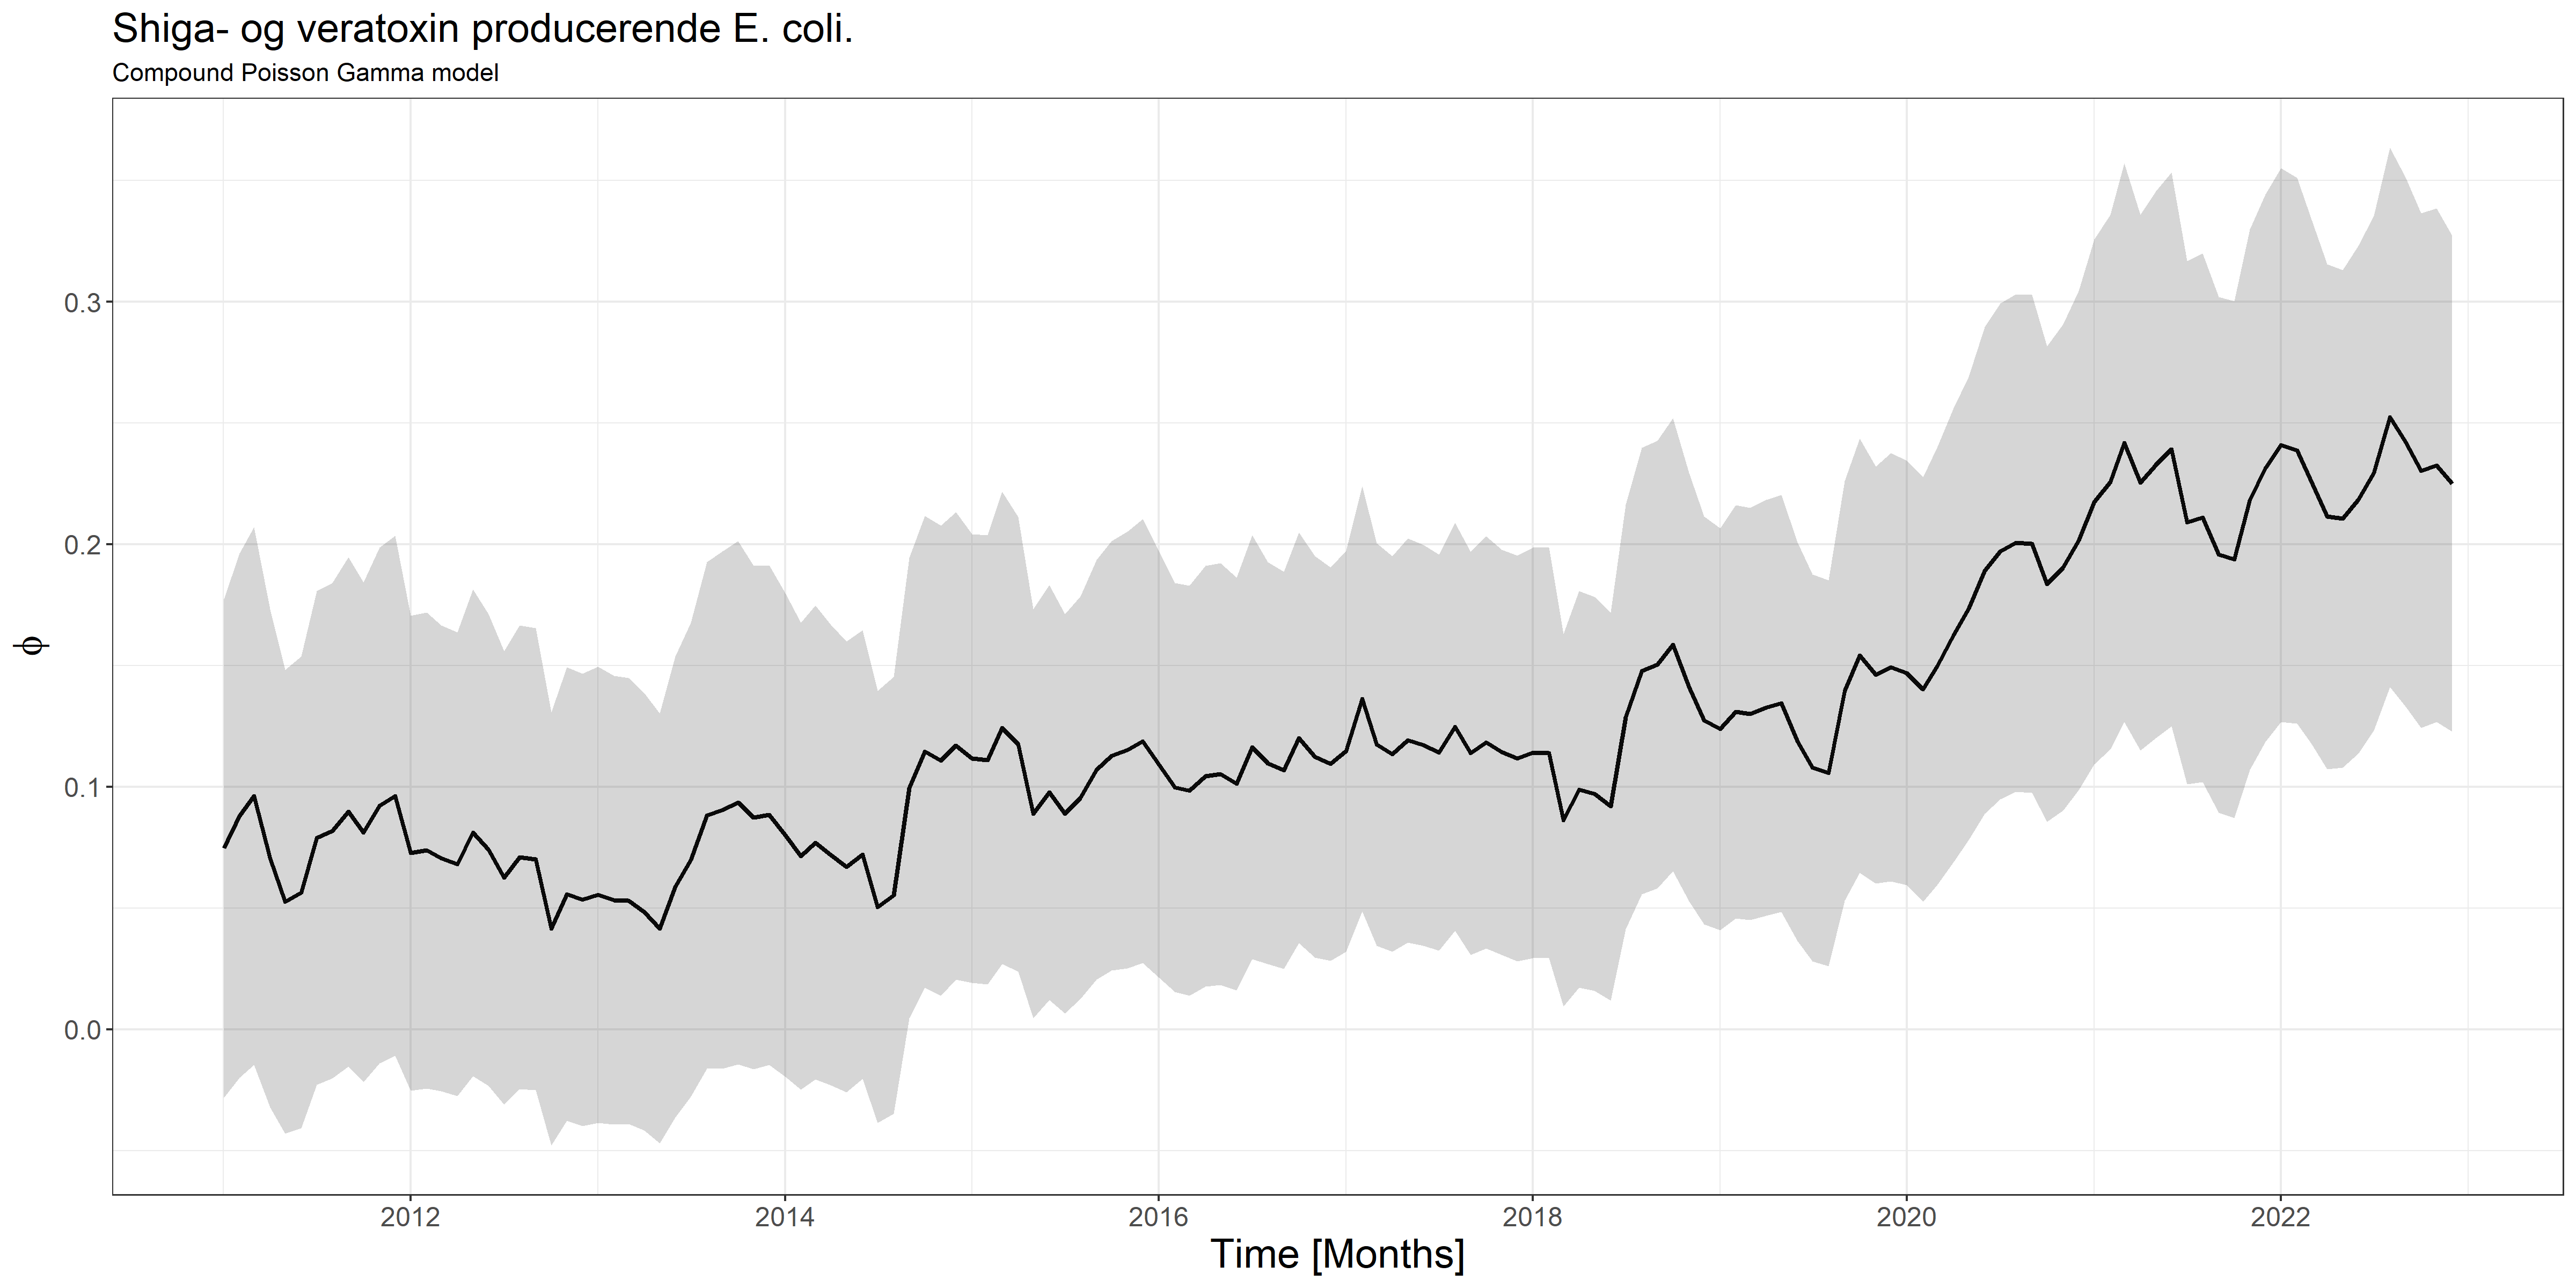
\includegraphics[width=1\linewidth]{../figures/phiSTECPoisGExclude}

\normalsize
\end{frame}

\begin{frame}{Threshold calculation}
\protect\hypertarget{threshold-calculation-1}{}
The critical value, \(C_\alpha\), is computed from the
\(1-\alpha\)-quantile of the reparametrized Gamma distribution with the
maximum-likelihood estimate for the variance, \(\hat\phi\).

\begin{equation}
  C_\alpha=\G(\boldsymbol{1}/\hat\phi,\hat\phi)_{1-\alpha}
\end{equation}
\end{frame}

\begin{frame}{Results - Out-of-sample random effects}
\protect\hypertarget{results---out-of-sample-random-effects-1}{}
\tiny

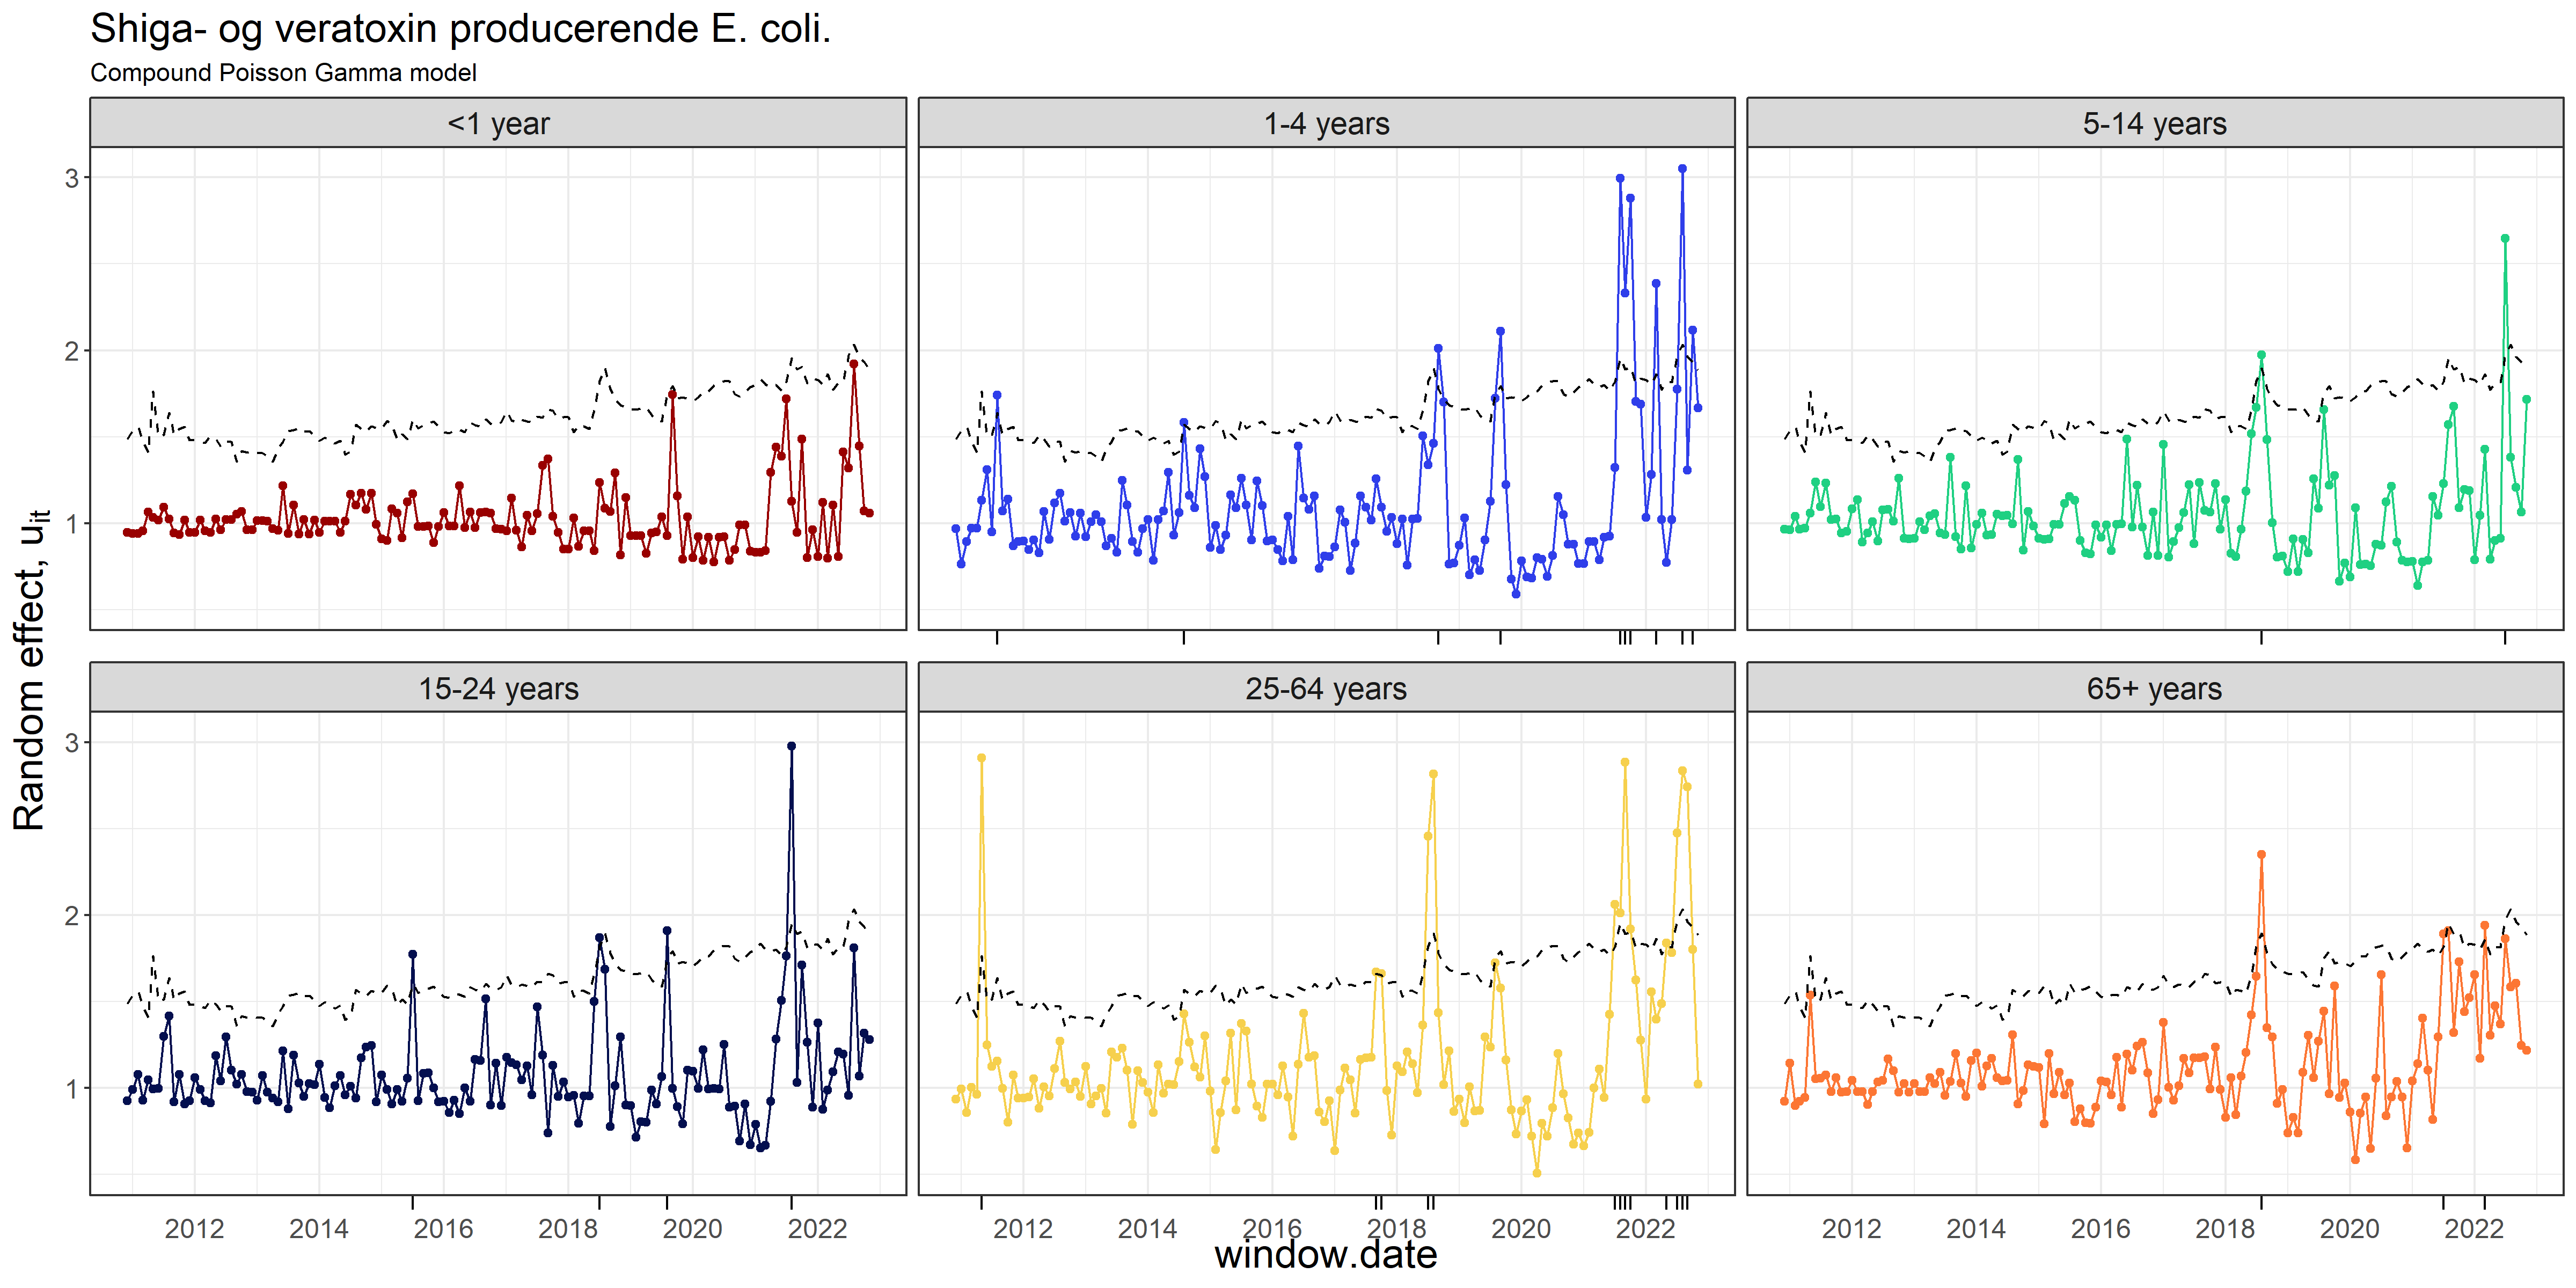
\includegraphics[width=1\linewidth]{../figures/windowedSTECPoisGExclude}

\normalsize
\end{frame}

\hypertarget{comparison-of-methods}{%
\section{Comparison of methods}\label{comparison-of-methods}}

\begin{frame}{Comparison of methods}
\tiny

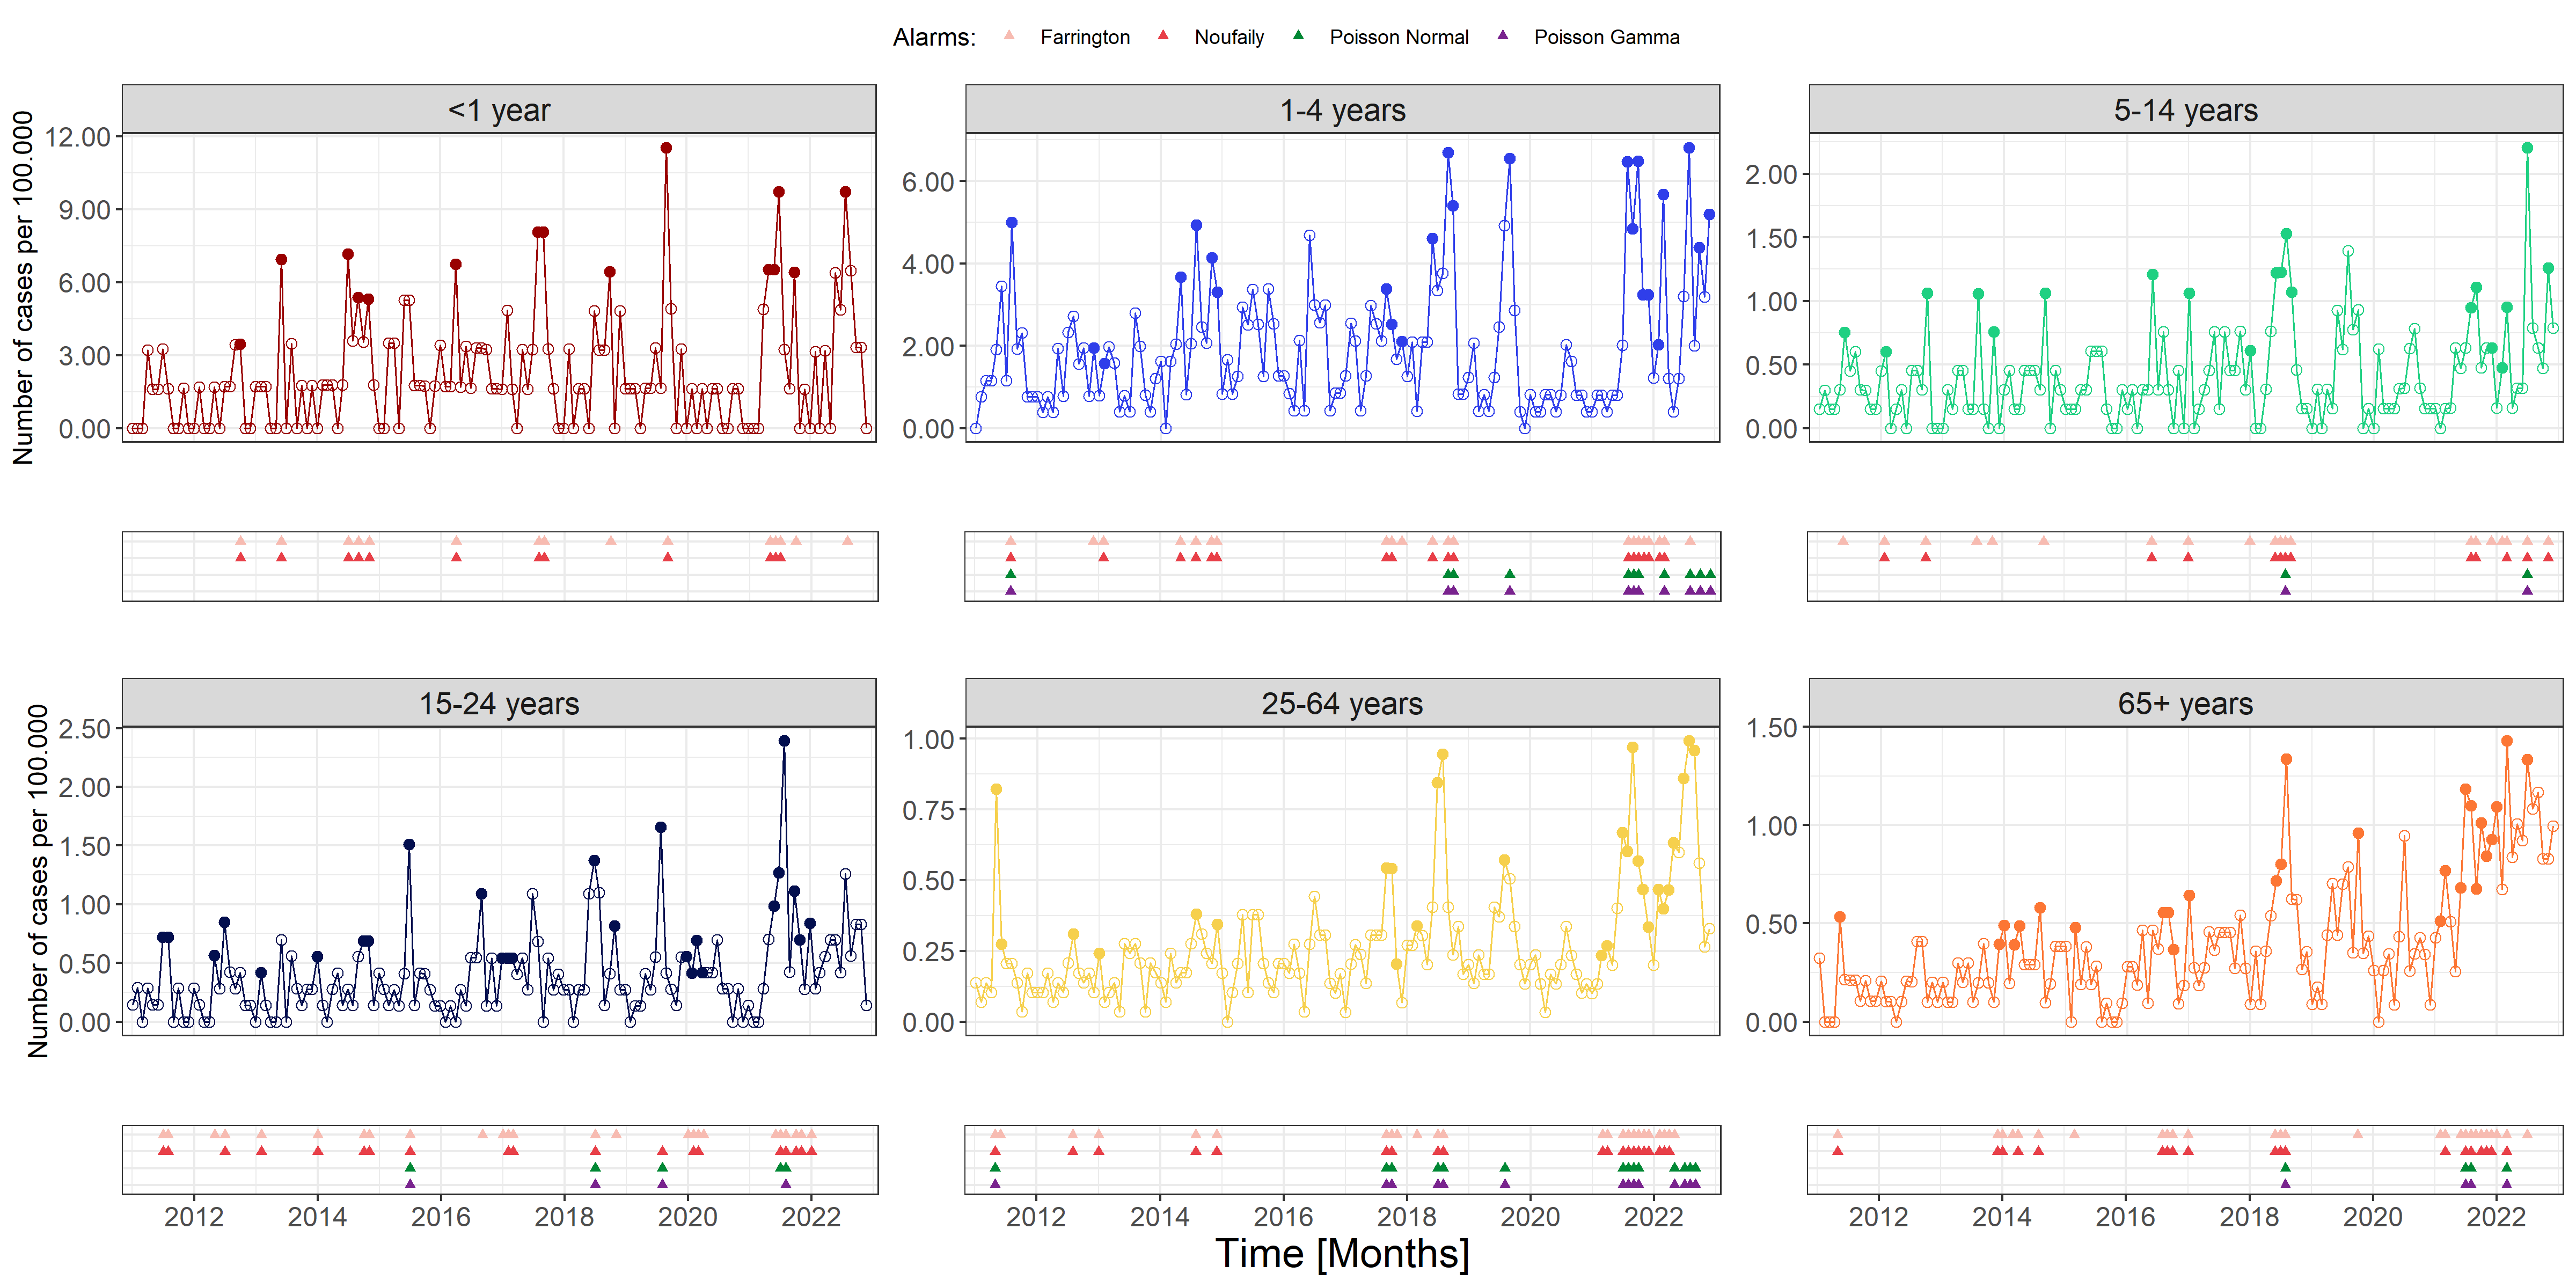
\includegraphics[width=1\linewidth]{../figures/compareMethodsDeluxe}

\normalsize
\end{frame}

\hypertarget{references}{%
\section{References}\label{references}}

\begin{frame}{References}
\printbibliography[heading=none]
\end{frame}

\hypertarget{appendix}{%
\section{Appendix}\label{appendix}}

\begin{frame}{Proof - Probability function for \emph{Y}}
\protect\hypertarget{proof---probability-function-for-y}{}
The probability function for the conditional distribution of \(Y\) for
given \(u\)

\begin{equation} \label{eq:pdfPois}
  f_{Y|u}(y;\lambda, u)=\frac{(\lambda u)^y}{y!} \exp (-\lambda u)
\end{equation}

and the probability density function for the distribution of \(u\) is

\begin{equation} \label{eq:pdfGamma}
  f_{u}(u;\phi)=\frac{1}{\phi \Gamma(1/\phi)} \bigg(\frac{u}{\phi}\bigg)^{1/\phi-1} \exp (-u/\phi)
\end{equation}
\end{frame}

\begin{frame}{Proof - Probability function for \emph{Y}}
\protect\hypertarget{proof---probability-function-for-y-1}{}
Given \eqref{eq:pdfPois} and \eqref{eq:pdfGamma}, the probability
function for the marginal distribution of \(Y\) is determined from

\begin{equation} \label{eq:marMix}
  \begin{aligned}
    g_{Y}(y;\lambda,\phi)&=\int_{u=0}^\infty f_{Y|u}(y;\lambda, u) f_{u}(u;\phi) \,du \\
    &=\int_{u=0}^\infty \frac{(\lambda u)^y}{y!} \exp (-\lambda u) \frac{1}{\phi \Gamma(1/\phi)} \bigg(\frac{u}{\phi}\bigg)^{1/\phi-1} \exp (-u/\phi) \,du\\
    &=\frac{\lambda^{y}}{y!\Gamma(1/\phi)\phi^{1/\phi}} \int_{u=0}^\infty u^{y+1/\phi-1} \exp \big(-u(\lambda \phi+1)/\phi\big) \,du
  \end{aligned}
\end{equation}
\end{frame}

\begin{frame}{Proof - Probability function for \emph{Y}}
\protect\hypertarget{proof---probability-function-for-y-2}{}
In \eqref{eq:marMix} it is noted that the integrand is the \emph{kernel}
in the probability density function for a Gamma distribution,
\(\G\big(y+1/\phi,\phi/(\lambda \phi+1)\big)\). As the integral of the
density shall equal one, we find by adjusting the norming constant that

\begin{equation}
  \int_{u=0}^\infty u^{y+1/\phi-1} \exp \bigg(-u/\Big(\phi/(\lambda \phi+1)\Big)\bigg) \,du = \frac{\phi^{y+1/\phi}\Gamma(y+1/\phi)}{(\lambda \phi + 1)^{y+1/\phi}}
\end{equation}

and then \eqref{eq:pdfMix} follows
\end{frame}

\begin{frame}{Proof - Conditional distribution of \emph{Y}}
\protect\hypertarget{proof---conditional-distribution-of-y}{}
The conditional distribution is found using Bayes Theorem

\begin{equation}
  \begin{aligned}
    g_{u}(u|Y=y)&=\frac{f_{y,u}(y,u)}{g_Y(y;\lambda, \phi)} \\
    &=\frac{f_{y|u}(y;u)g_{u}(u)}{g_{Y}(y;\lambda,\phi)} \\
    &=\frac{1}{g_{Y}(y;\lambda,\phi)}\bigg(\frac{(\lambda u)^y}{y!} \exp (-\lambda u) \frac{1}{\phi \Gamma(1/\phi)} \bigg(\frac{u}{\phi}\bigg)^{1/\phi-1} \exp (-u/\phi)\bigg) \\
    &\propto u^{y+1/\phi-1} \exp \big(- u(\lambda\phi+1)/\phi\big)
  \end{aligned}
\end{equation}

We identify the \emph{kernel} of the probability density function

\begin{equation}
  u^{y+1/\phi-1} \exp (- u(\lambda\phi+1)/\phi)
\end{equation}

as the kernel of a Gamma distribution,
\(\G(y+1/\phi,\phi/(\lambda\phi+1))\)
\end{frame}


\end{document}
